\documentclass[12pt]{article}
\usepackage[utf8]{inputenc}
\usepackage[top=3cm,right=2.5cm,bottom=2.5cm,left=3cm]{geometry}
\usepackage{amsmath}
\usepackage{amsfonts}
\usepackage{bm}
\usepackage{upgreek}
\usepackage{color}
\usepackage{hyperref}
\usepackage{graphicx}
\usepackage{subcaption}
\usepackage{tikz}
\usepackage{forest}
\usepackage[toc,title,page]{appendix}
\usepackage[colorinlistoftodos, color=blue!20!white, bordercolor=gray,
textsize=tiny,textwidth=0.8in]{todonotes}

\definecolor{folderbg}{RGB}{124,166,198}
\definecolor{folderborder}{RGB}{110,144,169}

\def\Size{4pt}
\tikzset{
  folder/.pic={
    \filldraw[draw=folderborder,top color=folderbg!50,bottom color=folderbg]
      (-1.05*\Size,0.2\Size+5pt) rectangle ++(.75*\Size,-0.2\Size-5pt);  
    \filldraw[draw=folderborder,top color=folderbg!50,bottom color=folderbg]
      (-1.15*\Size,-\Size) rectangle (1.15*\Size,\Size);
  }
}

\usepackage{comment}


\newcommand{\tr}{{\sf T}} % trace of a matrix
\newcommand{\code}[1]{\texttt{#1}}

\newcommand{\Frc}{\mbox{\rm Fr}_c} % Froude number
\newcommand{\Ma}{\mbox{\rm Ma}} % Mach number
\newcommand{\Rec}{\mbox{\rm Re}_c} % Reyolds number
\newcommand{\Rep}{\mbox{\rm Re}_p} % Particle Reyolds number
\newcommand{\Prand}{\mbox{\rm Pr}} % Prandtl number
\newcommand{\Sc}{\mbox{\rm Sc}} % Schmidt number
\newcommand{\Atw}{\mbox{\rm At}} % Schmidt number

\newcommand{\jcode}{\code{jCODE}~}
\newcommand{\inp}{\code{input}~}
\newcommand{\rootdir}{\code{\MakeLowercase{\jcode}}}
\newcommand{\github}{\url{https://github.com/jessecaps/jCODE}}
\newcommand{\binary}{\code{jcode}}
\newcommand{\alert}[1]{{\color{red}#1}}
\def \gxy{\mathcal{G}\!\left( | \bm{x}-\bm{y} |\right)}
\def \gxi{\mathcal{G}\!\left( | \bm{x}-\bm{x}_p^{(i)} | \right)}
\def \gxp{\mathcal{G}\!\left( | \bm{x}-\bm{x}_p | \right)}


\title{$\jcode$ Manual}
\author{}
%\date{}

\begin{document}

\maketitle

\tableofcontents

\section{Introduction}
$\jcode$ is a high-performance, Fortran/MPI-based code that solves the viscous compressible Navier--Stokes equations on a structured curvilinear grid. The underlying numerical discretization was adapted from the code written by Dr. Ramanathan Vishnampet~\cite{vishnampet2015exact}. The code is developed and maintained by the Capecelatro Research Group at the University of Michigan. It features a range of models and methods designed for solving turbulent reacting multiphase flows. Various features include:
\begin{itemize}
\item High-order energy-stable discretization based on summation-by-parts finite differences
\item Lagrangian particle tracking with two-way coupling for mass, momentum, and heat transfer between phases
\item Immersed boundary method for treatment of complex geometries
\item Shock capturing based on localized artificial dissipation
\item Discrete adjoint method for obtaining precision-limited sensitivity gradients
\end{itemize}

This manual provides the necessary details for acquiring the code, compilation instructions, and several representative example cases. The following section will provide a brief description of the underlying physical models and numerical discretization. Further information can be found in the papers referenced throughout the document.

\section{Physical model}
\subsection{Non-dimensionalization \label{sec:nondimensional}}
The code uses the following variables for non-dimensionalization: $\rho_\infty^*$ (density), $c_\infty^*$ (the speed of sound), $\mu_\infty^*$ (viscosity), $C_{p,\infty}^{\star}$ (the heat capacity), and $L^*$, a length scale. For multi-component flows, the molecular weight $W_\infty^\star$ is also used. The superscript $\star$ denotes a dimensional quantity and subscript $\infty$ represents a reference quantity. With this, the non-dimensional variables are:
\begin{alignat*}{3}
x_i &= \frac{x_i^{\star}}{L^{\star}}, &{}u_i ={}& \frac{u_i^{\star}}{c_{\infty}^{\star}},  &t=& \frac{t^{\star}}{L^{\star}/c_{\infty}^{\star}},  \\
\rho &= \frac{\rho^{\star}}{\rho_{\infty}^{\star}},   &{}p={}& \frac{p^{\star}}{\rho_{\infty}^{\star} {c_{\infty}^{\star}}^2 }, &{}E={}&\frac{E^{\star}}{ {c_{\infty}^{\star}}^2 } \\
C_{p,k} &=  \frac{C_{p,k}^{\star}}{C_{p,\infty}^{\star}}, &{}W_k ={}& \frac{W_{k}^{\star}}{W_{\infty}^{\star}}, &\mu = &\frac{\mu^{\star}}{\mu_{\infty}^{\star}} \\
T &= \frac{T^{\star}}{{c_{\infty}^{\star}}^2 / C_{p,\infty}^{\star}}, &{}T={}&\frac{T^{\star}}{(\gamma-1)T_{\infty}^{\star}}, &{}\lambda ={}& \frac{\lambda^{\star}}{\mu_{\infty}^{\star}}
\end{alignat*}
\begin{comment}
\begin{align}
x_i &= \frac{x_i^{\star}}{L^{\star}}, \quad
u_i = \frac{u_i^{\star}}{c_{\infty}^{\star}}, \quad t = \frac{t^{\star}}{L^{\star}/c_{\infty}^{\star}}
\nonumber\\  \rho &= \frac{\rho^{\star}}{\rho_{\infty}^{\star}},  \quad p = \frac{p^{\star}}{\rho_{\infty}^{\star} {c_{\infty}^{\star}}^2 }, \quad E = \frac{E^{\star}}{ {c_{\infty}^{\star}}^2 }, 
\nonumber \\
C_{p,k} &= W_k^{-1} = \frac{C_{p,k}^{\star}}{C_{p,\infty}^{\star}} = \frac{W_{\infty}^{\star}}{W_{k}^{\star}}, \quad T = \frac{T^{\star}}{{c_{\infty}^{\star}}^2 / C_{p,\infty}^{\star}}=\frac{T^{\star}}{(\gamma-1)T_{\infty}^{\star}}, 
\nonumber \\
\mu &= \frac{\mu^{\star}}{\mu_{\infty}^{\star}}, \quad \lambda = \frac{\lambda^{\star}}{\mu_{\infty}^{\star}},
\end{align}
\end{comment}
where $x_i$ and $u_i$ are the location and velocity in the $i$-th direction, respectively, $\rho$ is the density, $p$ is the pressure, $E$ is the total energy per unit mass, $\gamma$ is the specific heat ratio, $C_{p,k}$ is the specific heat at constant pressure for species $k$, $W_k$ is the molecular weight of species $k$, and $\mu$ and $\lambda$ are the first and second viscosity coefficients, respectively.

The relevant non-dimensional numbers defined in \jcode are
\begin{align}\label{No_ndj}
\Rec = \frac{\rho_{\infty}^{\star} c_{\infty}^{\star} L^{\star} }{\mu_{\infty}^{\star}},  \quad \Pr = \frac{C_{p,\infty}^{\star} \mu^{\star}}{k^{\star}}, \quad \Sc_k = \frac{\mu^{\star}}{\rho^{\star}D_k^{\star}}, \quad \Frc = \frac{{c_{\infty}^{\star}}^2}{g^{\star} L^{\star}},
\end{align}
where $g^\star$ is the magnitude of gravity and $D_k^{\star}$ denotes the mass diffusivity of species $k$. % It is assumed that $ \rho^{\star} D_k^{\star} $ and $ k^{\star}/C_p^{\star}$ are proportional to $T^n$, such that $\Pr$ and $\Sc_k$ are constant.

\subsection{Governing equations and discretization\label{sec:Equations}}
The code solves the viscous compressible Navier--Stokes equations with options to include multiple species, Lagrangian particles, and/or immersed boundaries. When two-way coupling between the fluid and particles is enabled, the code solves the volume-filtered equations with appropriate source terms~\cite{shallcross2020volume}. Details on the fluid-phase equations are given in Sec.~\ref{sec:gas}, the particle equations of motion are provided in Sec.~\ref{sec:solid}, and details on two-way coupling can be found in Sec.~\ref{sec:twoway}.

\subsubsection{Gas-phase description \label{sec:gas}}
The conserved variables are density $\rho$, momentum in the $i$-th direction $\rho u_i$, total energy $\rho E$, and mass fraction for species $k$, $\rho Y_k$ for $k=1,\ldots,N$ with $N$ denoting the total number of species.
%The governing equations for the gas-phase can be written as
%\begin{align}
%\label{eq:rho}
%\frac{\partial \rho}{\partial t} + \frac{\partial \left( \rho u_j \right) }{\partial x_j} &=  S_{\rho}, 
%\\\label{eq:ui}
%\frac{\partial \left( \rho u_i \right)}{\partial t} + \frac{\partial}{\partial x_j}\left( \rho u_i u_j + p\delta_{ij} - \tau_{ij} \right) &= S_{\rho u_i}, 
%\\\label{eq:E}
%\frac{\partial \left( \rho E \right)}{\partial t} + \frac{\partial}{\partial x_j}\left[\left( \rho E + p \right) u_j + q_j - u_i\tau_{ij} \right] &= S_{\rho E},
%\\\label{eq:Y}
%\frac{\partial \left( \rho Y_n \right)}{\partial t} + \frac{\partial}{\partial x_j} \left( \rho u_j Y_n + f_n^{V} \right)&= S_{\rho Y}, \ \text{for}\ n=1,2,\cdots, N-1 ,
%\end{align}
The governing equations for the gas-phase can be written compactly as
\begin{align}\label{eq:compact_N_S}
\frac{\partial \bm{Q}}{\partial t}+\frac{\partial \bm{F}_i}{\partial x_i}=\bm{S},
\end{align}
where $\bm{Q}=[\rho, \ \rho u_1, \ \rho u_2, \ \rho u_3, \ \rho E, \ \rho Y_1, \ \cdots, \  \rho Y_{N-1}]^\tr$ is a vector containing the conservative variables, $\bm{F}_i = \bm{F}^I_i - \textbf{F}^V_i$ is the flux vector containing inviscid $\bm{F}^I_i$ and viscous $\bm{F}^V_i$ effects, and $\bm{S}$ is a vector of volumetric source terms (e.g., due to gravity, two-way coupling with particles, or combustion). The inviscid and viscous fluxes in direction $i$ are
\begin{align}\label{F_S_1}
\bm{F}^I_i=\begin{bmatrix}
\rho u_i \\
\rho u_1 u_i + p \delta_{i1} \\
\rho u_2 u_i + p \delta_{i2} \\
\rho u_3 u_i + p \delta_{i3} \\
u_i(\rho E + p ) \\
\rho Y_1 u_i\\
\vdots\\
\rho Y_{N-1} u_i
\end{bmatrix},
\quad \bm{F}^V_i=\begin{bmatrix}
0 \\
\tau_{1i} \\
\tau_{2i} \\
\tau_{3i} \\
u_j \tau_{ij} - q_i \\
f^V_1\\
\vdots\\
f^V_{N-1}
\end{bmatrix}.
\end{align}
where $\tau_{ij}$ denotes  non-dimensional viscous stress tensor, given by
\begin{align}\label{tau}
\tau_{ij}=\frac{\mu}{\Rec}\left(\frac{\partial u_i}{\partial x_j}+\frac{\partial u_j}{\partial x_i}\right)+\frac{\lambda}{\Rec}\frac{\partial u_k}{\partial x_k}\delta _{ij}.
\end{align}
The non-dimensional heat flux is given by
\begin{align}\label{q}
q_i=-\frac{\mu}{\Rec \Pr}\frac{\partial T}{\partial x_i} - \frac{\mu T}{\Rec}\sum \limits_{k=1}^N \frac{1}{W_k \Sc_k}\frac{\partial Y_k}{\partial x_i},
\end{align}
and the non-dimensional mass flux is given by
\begin{align}\label{f^V_n}
f^V_k=\frac{\mu}{\Rec \Sc_k}\frac{\partial Y_k}{\partial x_i}, \quad \text{for} \ k = 1, \dots, N-1.
\end{align}
Pressure and temperature are dependent variables that are determined according to thermodynamic relations and an equation of state, given by
\begin{align}\label{p_T}
p =  \left(\gamma -1\right) \left( \rho E - \frac{1}{2}\rho u_i u_i \right)\quad{\rm and}\quad
T = \frac{\gamma}{\gamma-1 } \frac{p W}{\rho},
\end{align}
where $W$ is the mixture molecular weight. For a single component fluid, $W=1$ and for a mixture, it is defined as
\begin{align}\label{W}
\frac{1}{W} = \sum \limits_{k=1}^N \frac{Y_k}{W_k}.
\end{align}
Finally, $\mu$ varies with temperature according to $\mu = [(\gamma -1)T]^n $, and $ \lambda=\mu _B - 2\mu/3$  where $ \mu _B = 0.6 \mu $  is the bulk viscosity.

The governing equations are discretized in generalized curvilinear coordinates. Physical coordinates $\bm{x}=(x_1,\,x_2,\,x_3)$ are transformed to computational coordinates $\bm{\xi}=(\xi_1,\,\xi_2,\,\xi_3)$ via
\begin{equation}
\bm{x}=X(\bm{\xi})\quad{\rm with\ inverse}\quad\bm{\xi}=\Xi_i(\bm{x}),
\end{equation}
so that $X^{-1}=\Xi$. The transformation Jacobian $J={\rm det}\left(\frac{\partial\xi_i}{\partial x_j}\right)$ is positive definite, and metrics are defined ${\rm M}_{ij}=J^{-1}\frac{\partial\xi_i}{\partial x_j}$ with $\frac{\partial {\rm M}_{ij}}{\partial\xi_i}=0$, so the transformed flow equations are 
\begin{equation}\label{eq:curvilinear}
\frac{\partial \bm{Q}}{\partial t}+J \frac{\partial}{\partial \xi_{i}}\left[\mathrm{M}_{i j}\left(\bm{F}_{j}^{I}-\bm{F}_{j}^{V}\right)\right]=\bm{S}.
\end{equation}
Derivatives $\partial/\partial\xi_i$ are approximated by a narrow-stencil finite-difference operator that satisfies the summation-by-part (SBP) property~\cite{strand1994summation}. This leads to $2s$-order centered-difference stencils at interior points and $s$-order accurate biased stencils near boundaries, with $s+1$ global accuracy.  To evaluate second and mixed derivatives, first derivative operators are applied consecutively, necessitating the use of artificial dissipation to damp the highest wavenumber components supported by the grid. High-order accurate SBP dissipation operators may be used to provide artificial dissipation with a diffusion coefficient that is a function of the local grid resolution~\cite{mattsson2004stable,vishnampet2015exact}. The boundary conditions are imposed weakly to ensure provable stability by employing the simultaneous-approximation-term (SAT) boundary treatment~\cite{carpenter1994time, vishnampet2015exact}. A list of available boundary conditions is provided in Sec.~\ref{input:patch}.

%Conservation of secondary quantities, such as kinetic energy, is necessary to achieve stable numerical simulations of turbulent flows.
Kinetic energy preservation is achieved using a skew-symmetric-type splitting of the inviscid flux in generalized curvilinear coordinates \cite{pirozzoli2011stabilized}, which provides nonlinear stability at low Mach number. The convective flux appearing in \eqref{eq:curvilinear} is expressed in split form as
\begin{equation}
\frac{\partial\rho\hat{u}_i\varphi}{\partial\xi_i}=\frac{1}{2}\frac{\partial\rho\hat{u}_i\varphi}{\partial\xi_i}+\frac{1}{2}\varphi\frac{\partial\rho\hat{u}_i}{\partial\xi_i}+\frac{1}{2}\rho\hat{u}_i\frac{\partial\varphi}{\partial\xi_i},
\end{equation}
where $\hat{u}_i={\rm M}_{ij}u_j$ is the contravariant velocity and $\varphi$ is a generic transported scalar, being unity for the continuity equation, $u_i$ for the momentum equation, and $H=E+p/\rho$ for the total energy equation. The pressure gradient term in the momentum equation is split in a similar fashion according to
\begin{equation}
\frac{\partial p {\rm M}_{ij}}{\partial \xi_i}=\frac{1}{2}\frac{\partial p {\rm M}_{ij}}{\partial \xi_i}+\frac{1}{2}p\frac{\partial {\rm M}_{ij}}{\partial \xi_i}+\frac{1}{2}{\rm M}_{ij}\frac{\partial p}{\partial \xi_i}.
\end{equation}

%%%%%%%%%%%%%%%%%%%%%%%%%%%%%%%%%%%%%%%%%%%%%%%%%%%%%%%%
\subsubsection{Particle-phase description \label{sec:solid}}
Particles are modeled as discrete entities that are tracked in a Lagrangian manner. The displacement and velocity of an individual particle $i$ are given by Newton's second law according to
\begin{equation}
\frac{ {\rm d} \bm{x}_{p}^{(i)}}{ {\rm d} t} = \bm{v}_p^{(i)}\quad{\rm and}\quad m_p \frac{ {\rm d} \bm{v}_{p}^{(i)}}{ {\rm d} t} = \bm{f}_{\rm inter}^{(i)} + \bm{f}^{(i)}_{\rm col},
\end{equation}
where  $m_p = \pi \rho_p d_p^3 / 6$ is the particle mass with $\rho_p$ the particle density, $\bm{f}_{\rm inter}^{(i)}$ accounts for fluid stresses at the particle surface, and $\bm{f}^{(i)}_{\rm col}$ accounts for particle-particle interactions (e.g., collisions). A soft-sphere collision model is used to handle particle-particle and particle-wall contact. Particles are treated as elastic and frictional with a coefficient of restitution and friction coefficient provided by the user. Collisions and handled efficiently using a nearest-neighbor detection algorithm~\cite{capecelatro2013euler}. Momentum exchange between the phases is decomposed into resolved and unresolved contributions, expressed as
\begin{equation}\label{eq:finter}
\bm{f}_{\rm inter}^{(i)}  = \mathcal{V}_p \nabla \cdot \left(- p \mathbb{I}+\bm{\tau}\right) + \bm{f}_{\rm drag}^{(i)},
\end{equation}
where $\mathcal{V}_p$ is the particle volume, and $\bm{f}_{\rm drag}^{(i)}$ can be handled using a variety of drag laws available in the code. A list of available drag models is provided in Sec.~\ref{input:particle}. Further details are provided in Appendix~\ref{app:drag}.

The evolution of particle temperature is expressed as
\begin{equation}\label{dtdt}
m_p C_{p,p} \frac{ {\rm d} T_p^{(i)}}{ {\rm d}t}=  \mathcal{V}_p \nabla \cdot \left( \frac{\mu}{\Rec \Pr}\nabla T \right) + \bm{q}_{\rm inter}^{(i)},
\end{equation}
where $T_p^{(i)}$ is the temperature of the $i$-th particle, $C_{p,p}$ is the ratio of particle-to-fluid heat capacity, and the sub-filtered heat flux, $\bm{q}_{\rm inter}^{(i)}$ is modeled using Nusselt number correlations. %Further details can be found in \cite{capecelatro2013euler,shallcross2020volume}.

\subsubsection{Two-way coupling \label{sec:twoway}}
When two-way coupling is enabled between the fluid and particle phases, the governing equations are modified to account for the fluid volume fraction, $0\le\alpha\le1$, and interphase exchange of mass, momentum, and energy. The fluid-phase conserved variables are modified as $\bm{Q}=[\alpha\rho, \ \alpha\rho u_1, \ \alpha\rho u_2, \ \alpha\rho u_3, \ \alpha\rho E, \ \alpha\rho Y_1, \ \cdots, \  \alpha\rho Y_{N-1}]^\tr$. Lagrangian particle data is projected to the mesh using a filter kernel $\mathcal{G}$ with a chosen size $\delta_f$. Interphase exchange terms are given by
\begin{equation}\label{eq:vf_project}
\text{Volume fraction:}\quad\alpha=1- \sum_{i = 1}^{N_p} \gxi \mathcal{V}_p,
\end{equation}
\begin{equation}
\text{Momentum exchange:}\quad\bm{\mathcal{F}} = -\sum_{i = 1}^{N_p} \gxi \bm{f}_{\rm inter}^{(i)},
\end{equation}
\begin{equation}
\text{Work due to momentum exchange:}\quad\bm{u}_p \cdot \bm{\mathcal{F}} = -\sum_{i = 1}^{N_p} \gxi \bm{v}_p^{(i)} \cdot \bm{f}_{\rm inter}^{(i)},
\end{equation}
\begin{equation}
\text{Heat exchange:}\quad\mathcal{Q} = - \sum_{i = 1}^{N_p} \gxi \bm{q}_{\rm inter}^{(i)}.
\end{equation}
A two step filtering approach~\cite{capecelatro2013euler} is employed that decouples the mesh size from particle diameter ratio in an efficient manner. First, particle data is sent to neighboring grid points via trilinear extrapolation. The solution is then diffused such that the filtered data is projected with characteristic size of $\delta_f$. To avoid restrictive time step constraints in the diffusion process, the latter step is solved implicitly via approximate factorization with a second order alternating direction implicit (ADI) scheme.

\subsection{Time integration}
A family of explicit Runge--Kutta (RK) time integration schemes are available in the code. This includes a first-order RK scheme (Euler method); second-order RK (predictor-corrector scheme); an optimal third-order total variation diminishing (TVD) RK method~\cite{gottlieb1998total}; and a standard fourth-order scheme (RK4). All modules employ the same time marching scheme (e.g., gas-phase equations, particles, immersed boundaries). However, at present, the adjoint solver is only implemented using the RK4 scheme.

\subsection{Adjoint method}
The adjoint of the perturbed and linearized governing equations can be solved in continuous or discrete form. The adjoint provides the sensitivity gradient of a quantity of interest $\mathcal{J}$ (referred to as the cost functional) to a chosen set of parameters $\bm{\theta}$ (also referred to as the control parameters in \jcode). A list of available cost functionals and control parameters is provided in Sec.~\ref{input:adjoint}. When the discrete adjoint method is used, the code returns an exact (to machine precision) sensitivity gradient consistent with the SBP-SAT discretization described in the previous section.

In general, we write the cost functional $\mathcal{J}$ as
\begin{equation}\label{Jdef}
\mathcal{J}(\bm{Q},\bm{\theta}) = \int_{t_1}^{t_2} \int_{\Omega} j(\bm{Q},\bm{\theta}) \, \text{d}\bm{x} \, \text{d} t,
\end{equation}
where $j(\bm{Q},\bm{\theta})$ is the the cost functional integrated in a target region $\Omega$ over duration $t_1$ to $t_2$. The change, or first variation, in $\delta\mathcal{J}$ is written as
\begin{equation}
\label{deltaJ}
\delta\mathcal{J}=\int_{t_1}^{t_2} \int_{\Omega} \left\{\left(\frac{\partial j}{\partial \bm{Q}}\right)^{\sf T} \, \delta \bm{Q} + \left(\frac{\partial j}{\partial \bm{\theta}}\right)^{\sf T} \, \delta \bm{\theta}\right\} \, \textrm{d}\bm{x} \, \textrm{d} t.
\end{equation}
Here, $\delta \bm{Q}$ represents linear perturbations to the flow solution due to variations in the parameters $\delta\bm{\theta}$ (which in general would require repeated simulations). The adjoint equations are formulated to eliminate the $\delta \bm{Q}$ dependence in \eqref{deltaJ}. To do this, we introduce the adjoint variable $\bm{Q}^\dagger$ as a Lagrange multiplier to enforce adherence to the governing equations \eqref{eq:curvilinear} as a constraint, written as
\begin{equation}
\mathcal{N}[\bm{Q};\bm{\theta}] = 0 \quad \text{where} \quad \mathcal{N}[\bm{Q};\bm{\theta}] = \frac{\partial\bm{Q}}{\partial t} + J \frac{\partial}{\partial \xi_i}\left[{\rm M}_{ij}\bm{F}_j(\bm{Q})\right] - \bm{S}(\bm{Q}, \bm{\theta}).
\label{vecN}
\end{equation}
Variations with respect to the flow solution $\bm{Q}$ result in a set of partial differential equations that describe the evolution of the adjoint variables
\begin{equation}\label{adjEq}
\mathcal{N}^\dagger[\bm{Q}^\dagger;\bm{Q}]=-\frac{\partial \bm{Q}^\dagger}{\partial t}-J\left[\mathcal{A}_i^{\sf T} \frac{\partial \bm{Q}^\dagger}{\partial\xi_i}+\mathcal{D}^{\sf T} \frac{\partial}{\partial\xi_j}\left(\mathcal{B}_{ij}^{\sf T} \frac{\partial \bm{Q}^\dagger}{\partial\xi_i} \right)\right]+\mathcal{D}^{\sf T} \mathcal{C}^{\sf T} \bm{Q}^\dagger = 0.
\end{equation}
Due to the the negative sign that appears in front of the time derivative, these equations have to be solved backward in time. The coefficient matrices $\mathcal{A}$, $\mathcal{B}$, $\mathcal{C}$, and $\mathcal{D}$ can be found in \cite{capecelatro2018adjoint}. Because the flow variables appear in the adjoint equations as coefficients, they must be available. A standard checkpointing scheme is utilized to do this efficiently.

Once the adjoint variables are solved for, the corresponding sensitivity gradient can be determined according to
\begin{equation}\label{gradient}
\frac{\delta\mathcal{J}}{\delta\bm{\theta}}=\int_{t_1}^{t_2}\int_\Omega \left(\frac{\partial j}{\partial \bm{\theta}}-\bm{Q}^{\dagger^{\sf T}}\frac{\partial \bm{S}}{\partial\bm{\theta}}\right)~\text{d}\bm{x}\,\text{d}t,
\end{equation}
with $\delta\mathcal{J}$ now directly related to $\delta \bm{\theta}$, independent of $\delta \bm{Q}$. Several optimization routines exist in the code that make use of this sensitivity gradient.

\section{Source code and compilation}
%This section outlines all the steps required to acquire, compile, and run the code: obtaining the source code (Section \ref{sec:source}, installing and compiling the software (Section \ref{sec:compile}).

\subsection{Obtaining the source code \label{sec:source}}
The code is currently managed via a Git repository stored on \github. It is freely available online. It is advised to create a fork of the main branch and work off of that, or simply download a copy of the source code to your local machine.

Once you have access to the source code, you will find that \jcode contains several directories. Their contents and a brief description are outlined in Fig.~\ref{fig:folders}.

\begin{figure}
\centering
\begin{scriptsize}
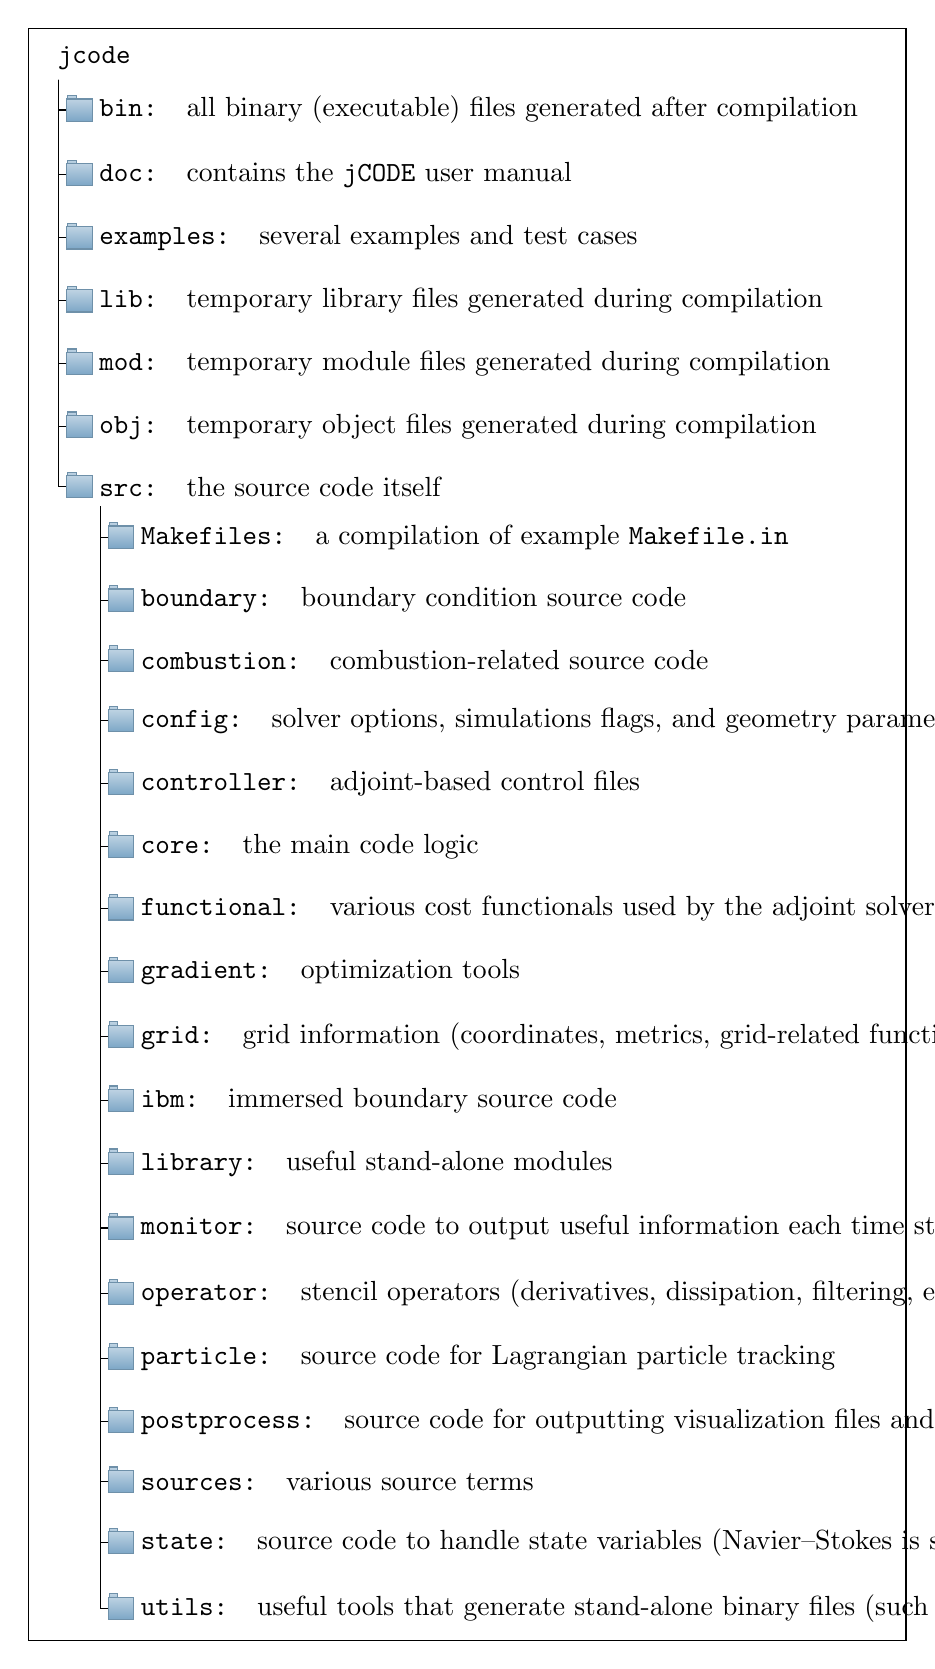
\begin{tikzpicture}
\node[draw, fill = white,text width=0.9\textwidth] at (0,0) {
\begin{forest}
  for tree={
    font=\ttfamily,
    grow'=0,
    child anchor=west,
    parent anchor=south,
    anchor=west,
    calign=first,
    inner xsep=7pt,
    edge path={
      \noexpand\path [draw, \forestoption{edge}]
      (!u.south west) +(7.5pt,0) |- (.child anchor) pic {folder} \forestoption{edge label};
    },
    before typesetting nodes={
      if n=1
        {insert before={[,phantom]}}
        {}
    },
    fit=band,
    before computing xy={l=15pt},
  }  
[jcode
  [bin: \textrm{all binary (executable) files generated after compilation}
  ]
    [doc: \textrm{contains the \jcode user manual}
  ]
  [examples: \textrm{several examples and test cases}
  ]
[lib: \textrm{temporary library files generated during compilation}
]
[mod: \textrm{temporary module files generated during compilation}
]
[obj: \textrm{temporary object files generated during compilation}
]
[src: \textrm{the source code itself}
  [Makefiles: \textrm{a compilation of example \code{Makefile.in}}
  ]
  [boundary: \textrm{boundary condition source code}
  ]
[combustion: \textrm{combustion-related source code} 
]
[config: \textrm{solver options, simulations flags, and geometry parameters}
]
[controller: \textrm{adjoint-based control files}
]
[core: \textrm{the main code logic}
]
[functional: \textrm{various cost functionals used by the adjoint solver}
]
[gradient: \textrm{optimization tools}
]
[grid: \textrm{grid information (coordinates, metrics, grid-related functions)}
]
[ibm: \textrm{immersed boundary source code}
]
[library: \textrm{useful stand-alone modules}
]
[monitor: \textrm{source code to output useful information each time step (timing, stats, etc.)}
]
[operator: \textrm{stencil operators (derivatives, dissipation, filtering, etc.)}
]
[particle: \textrm{source code for Lagrangian particle tracking}
]
[postprocess: \textrm{source code for outputting visualization files and statistics}
]
[sources: \textrm{various source terms}
]
[state: \textrm{source code to handle state variables (Navier--Stokes is solved here)}
]
[utils: \textrm{useful tools that generate stand-alone binary files (such as init\_flow)}
]
]
    ]
\end{forest}};
\end{tikzpicture}
\end{scriptsize}
\caption{Summary of the \jcode\ file structure}
\label{fig:folders}
\end{figure}

\newpage

\subsection{Compilation details \label{sec:compile}}
In order to install \jcode\ you must have Fortran 90 compilers and MPI installed. Once these are installed, you may install the CFD code itself. This section describes how to complete the download, configuration, and installation.

The source code of $\jcode$ is available in the \code{src} directory. The code requires two files to compile: \code{Makefile} and \code{Makefile.in}.
The file named \code{Makefile} is generic and architecture/compiler independent. It does not require modification. The file named \code{Makefile.in} contains architecture/compiler information that will need to be written for your particular hardware. There is no default \code{Makefile.in} file when you download the code for the first time. However, you can find templates for different architectures and compilers in the \code{Makefiles} directory. 
Chose an appropriate template from the \code{Makefiles} directory and copy it into \code{src}.
Ensure that \code{Makefile.in} is adapted to your architecture and set of compilers. Modify the following section of \code{Makefile.in} to match your local installation locations. 

\vspace{1em}
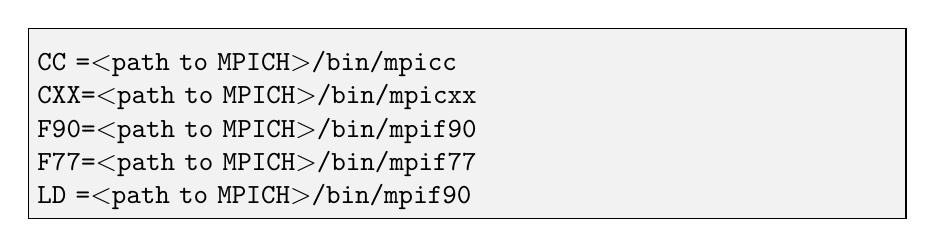
\begin{tikzpicture}
\node[draw, fill = gray!10,text width=0.9\textwidth] at (0,0) {\\\code{CC =$<$path to MPICH$>$/bin/mpicc}\\
\code{CXX=$<$path to MPICH$>$/bin/mpicxx}\\
\code{F90=$<$path to MPICH$>$/bin/mpif90}\\
\code{F77=$<$path to MPICH$>$/bin/mpif77}\\
\code{LD =$<$path to MPICH$>$/bin/mpif90}};
\end{tikzpicture}
\vspace{1em} 

\subsubsection*{Choosing the type of compilation}
The following compilation commands are executed from the command line while you are in the same folder as \code{Makefile.in}. \\

\noindent \code{make opt}: This target is generally for production runs, enables all optimization flags and the code will run the fastest. It is the most general way of compiling the code. \\

\noindent \code{make debug}: Use this target to compile the code with all debug flags enabled (additional flags can be added in \code{Makefile.in} if desired). Depending on the set of compilers, these flags might include: detection of unused variables, uninitialized variables, out-of bounds arrays, unassociated pointers, etc. If you suspect a bug in the code this is a good starting place for finding it. Note, the code will run $\sim4\times$ slower compared to optimized mode. \\

\noindent \code{make clean}:
Use this target if you want to remove all modules (.mod in \code{mod}), all object files (.o in \code{obj}), and all libraries (.a in \code{lib}) generated during compilation of the main source code. If the code is already compiled, you must run \code{make clean} before compiling in a different mode. \\

\noindent \code{make distclean}:
This will remove all temporary files associated with the \code{utils} directory. \\

\noindent It is good practice to start a new build with the following commands: 

\vspace{1em}
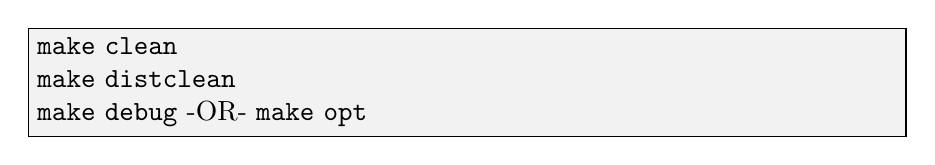
\begin{tikzpicture}
\node[draw, fill = gray!10,text width=0.9\textwidth] at (0,0) {
\code{make clean}\\
\code{make distclean}\\
\code{make debug} -OR- \code{make opt}};
\end{tikzpicture}
\vspace{1em} \\
Note that compilation might take up to 10 minutes on certain machines. After the code is compiled, a number of executable files can be found in the \code{bin} directory.

\section{Input deck}\label{sec:input_deck}
\inp\ is a text file that specifies the parameters used during initialization and run time.  Comments begin with either \# or !.  Empty lines are permitted. The `initialization parameters' are only read when \code{init\_flow} is executed. All other parameters are read during the execution of \jcode itself. The following convention is used in this section:

\vskip0.5\baselineskip
\noindent
\begin{tabular}{ll}
	\texttt{PARAMETER : DBLE} & The value of \texttt{PARAMETER} is a double precision number \\
	\texttt{PARAMETER : INT} & The value of \texttt{PARAMETER} is an integer \\
	\texttt{PARAMETER : STRING} & The value of \texttt{PARAMETER} is a character string \\
	\texttt{PARAMETER : LOGICAL} & The value of \texttt{PARAMETER} is a Fortran logical, \texttt{.true.} or \texttt{.false.} \\
    \texttt{PARAMETER : A B C } & The value of \texttt{PARAMETER} is an array and can be of mixed data types
\end{tabular}

\subsection{Initialization parameters}
\vskip\baselineskip
\noindent
\begin{verbatim}
# Initialization parameters ############################################
\end{verbatim}

\vskip\baselineskip
\noindent
\begin{minipage}{0.55\textwidth}
\begin{verbatim}
simulation name : STRING
\end{verbatim}
\end{minipage}
\hfill
\begin{minipage}{0.4\textwidth}
Determine the type of simulation. Examples will be given in the following section.
\end{minipage}

\vskip\baselineskip
\noindent
\begin{minipage}{0.55\textwidth}
\begin{verbatim}
! Grid size
nx : INT
ny : INT
nz : INT
\end{verbatim}
\end{minipage}
\hfill
\begin{minipage}{0.4\textwidth}
Specify the number of grid points in each direction.
\end{minipage}

\vskip\baselineskip
\noindent
\begin{minipage}{0.55\textwidth}
\begin{verbatim}
! Domain size
Lx : INT
Ly : INT
Lz : INT
\end{verbatim}
\end{minipage}
\hfill
\begin{minipage}{0.4\textwidth}
Specify the domain size in each direction.
\end{minipage}

\vskip\baselineskip
\noindent
\begin{minipage}{0.55\textwidth}
\begin{verbatim}
curvilinear domain : LOGICAL
\end{verbatim}
\end{minipage}
\hfill
\begin{minipage}{0.4\textwidth}
Determine whether curvilinear coordinates should be used.
\end{minipage}

\vskip\baselineskip
\noindent
\begin{minipage}{0.55\textwidth}
\begin{verbatim}
periodicity type in x : STRING
periodicity type in y : STRING
periodicity type in z : STRING
\end{verbatim}
\end{minipage}
\hfill
\begin{minipage}{0.4\textwidth}
Specify the periodicity type in direction \code{x}, \code{y}, or \code{z}. Options include \code{plane}, \code{overlap}, or \code{polar},  If not specified the default is \code{none}.
\end{minipage}

\vskip\baselineskip
\noindent
\begin{minipage}{0.55\textwidth}
\begin{verbatim}
! Initialization files
init grid file     : STRING
init solution file : STRING
\end{verbatim}
\end{minipage}
\hfill
\begin{minipage}{0.4\textwidth}
Specify the name for the grid file and solution file that will be written. By default, they are \code{grid} and \code{data.init}, respectively.
\end{minipage}

\subsection{Boundary conditions and patches}\label{input:patch}
\vskip\baselineskip
\noindent
\begin{verbatim}
# Boundary conditions and patches #######################################
\end{verbatim}

%\vskip\baselineskip
%\noindent
%\begin{minipage}{0.55\textwidth}
%\begin{verbatim}
%! Penalty parameters
%default viscous penalty amount : DBLE
%default sponge amount          : DBLE
%\end{verbatim}
%\end{minipage}
%\hfill
%\begin{minipage}{0.4\textwidth}
%Specify the values for viscous boundary penalty and sponge strength. By default they are 1.0 and 0.2, respectively.
%\end{minipage}

\vskip\baselineskip
\noindent
\begin{minipage}{0.3\textwidth}
\begin{verbatim}
! Patches :
! Name            Type    normDir   iMin  iMax   jMin  jMax   kMin  kMax
! -----------------------------------------------------------------------
  STRING          STRING  INT       INT   INT    INT   INT    INT   INT
\end{verbatim}
\end{minipage}

\vskip\baselineskip
\noindent
\hfill
\begin{minipage}{1.0\textwidth}
Grid patches are used in the code to execute specific functions within subregions of the domain (such as boundary conditions). \code{Name} can be any unique string. \code{Type} specifies which patch to use. A list of patch types can be found below. \code{normDir} represents the outward normal direction from the surface into the domain (when applied to domain boundaries), which can be either $\pm 1$, $\pm 2$ or $\pm 3$. \code{iMin, iMax, jMin, jMax, kMin, kMax} specify the region where the patch will be active. A negative value represents the number of grid points from the end. For example \code{iMin = 1, iMax = -1} will make the patch active across all grid points in the $x$-direction.
\end{minipage}

\vskip\baselineskip
\noindent
\begin{minipage}{0.55\textwidth}
\begin{verbatim}
SAT_FAR_FIELD
\end{verbatim}
\end{minipage}
\hfill
\begin{minipage}{0.45\textwidth}
Inflow/outflow characteristic boundary condition. Must be defined as a surface in 3D or a line in 2D.
\end{minipage}

\vskip\baselineskip
\noindent
\begin{minipage}{0.55\textwidth}
\begin{verbatim}
SAT_SLIP_WALL
\end{verbatim}
\end{minipage}
\hfill
\begin{minipage}{0.45\textwidth}
No penetration boundary condition. Must be defined as a surface in 3D or a line in 2D.
\end{minipage}

\vskip\baselineskip
\noindent
\begin{minipage}{0.55\textwidth}
\begin{verbatim}
SAT_ISOTHERMAL_WALL
\end{verbatim}
\end{minipage}
\hfill
\begin{minipage}{0.45\textwidth}
No-slip isothermal boundary condition. Must be defined as a surface in 3D or a line in 2D.
\end{minipage}

\vskip\baselineskip
\noindent
\begin{minipage}{0.55\textwidth}
\begin{verbatim}
SAT_ADIABATIC_WALL
\end{verbatim}
\end{minipage}
\hfill
\begin{minipage}{0.45\textwidth}
No-slip adiabatic wall boundary condition. Must be defined as a surface in 3D or a line in 2D.
\end{minipage}

\vskip\baselineskip
\noindent
\begin{minipage}{0.55\textwidth}
\begin{verbatim}
SPONGE
\end{verbatim}
\end{minipage}
\hfill
\begin{minipage}{0.45\textwidth}
Used to dampen the solution to a specified target solution near the boundary. Defined as a volume in 3D and an area in 2D.
\end{minipage}

\vskip\baselineskip
\noindent
\begin{minipage}{0.55\textwidth}
\begin{verbatim}
VISUALIZATION
\end{verbatim}
\end{minipage}
\hfill
\begin{minipage}{0.45\textwidth}
Used to define a specific region to write visualization files. If not specified, the post processing routine will output data of the entire grid size.
\end{minipage}

\vskip\baselineskip
\noindent
\begin{minipage}{0.55\textwidth}
\begin{verbatim}
ACTUATOR
\end{verbatim}
\end{minipage}
\hfill
\begin{minipage}{0.45\textwidth}
The control region used during an adjoint run. Must be defined as a volume in 3D and an area in 2D.
\end{minipage}

\vskip\baselineskip
\noindent
\begin{minipage}{0.55\textwidth}
\begin{verbatim}
COST_TARGET
\end{verbatim}
\end{minipage}
\hfill
\begin{minipage}{0.45\textwidth}
The target region used to compute the cost functional during an adjoint run. Must be defined as a volume in 3D and an area in 2D.
\end{minipage}


%%%%%%%%%%%%%%%%%%%%%%%%%%%%%%%%%%%%%%%
%%%%%%%%%%%%%%%%%%%%%%%%%%%%%%%%%%%%%%%
%%%%%%%%%%%%%%%%%%%%%%%%%%%%%%%%%%%%%%%
\subsection{General runtime parameters}


\vskip\baselineskip
\noindent
\begin{minipage}{0.55\textwidth}
\begin{verbatim}
! Files
data overwrite : LOGICAL
\end{verbatim}
\end{minipage}
\hfill
\begin{minipage}{0.45\textwidth}
Specifies if the data file is overwritten during runtime. The default is false for adjoint simulations and is true otherwise.
\end{minipage}


\vskip\baselineskip
\noindent
\begin{minipage}{0.45\textwidth}
\begin{verbatim}
use serial io : LOGICAL
\end{verbatim}
\end{minipage}
\hfill
\begin{minipage}{0.45\textwidth}
Specifies if processors read/write data to separate files (serial I/O) or to a single file (parallel I/O). The default is false.
\end{minipage}



\vskip\baselineskip
\noindent
\begin{minipage}{0.55\textwidth}
\begin{verbatim}
grid file : STRING
solution file to read : STRING
\end{verbatim}
\end{minipage}
\hfill
\begin{minipage}{0.45\textwidth}
Specifies the name of the grid and solution file to be read by \jcode (required).
\end{minipage}

\vskip\baselineskip
\noindent
\begin{minipage}{0.45\textwidth}
\begin{verbatim}
solution file to write : STRING
\end{verbatim}
\end{minipage}
\hfill
\begin{minipage}{0.45\textwidth}
Specifies the name for writing the solution file (required).
\end{minipage}


\vskip\baselineskip
\noindent
\begin{minipage}{0.45\textwidth}
\begin{verbatim}
save interval : INT
\end{verbatim}
\end{minipage}
\hfill
\begin{minipage}{0.45\textwidth}
Specifies the frequency for writing solution files.
\end{minipage}


\vskip\baselineskip
\noindent
\begin{minipage}{0.45\textwidth}
\begin{verbatim}
! Target state
use target state      : LOGICAL
target state file     : STRING
\end{verbatim}
\end{minipage}
\hfill
\begin{minipage}{0.45\textwidth}
Specifies if a target file is provided for setting the boundary values (the default is true).
\end{minipage}

\vskip\baselineskip
\noindent
\begin{minipage}{0.55\textwidth}
\begin{verbatim}
! Manual processor decomposition
use manual domain decomposition : LOGICAL
\end{verbatim}
\end{minipage}
\hfill
\begin{minipage}{0.4\textwidth}
Choose whether or not manual processor decomposition should be used. The default value is false. If false, the code will automatically determine how best to distribute the processors across the domain.
\end{minipage}

\vskip\baselineskip
\noindent
\begin{minipage}{0.55\textwidth}
\begin{verbatim}
processor decomposition : INT INT INT
\end{verbatim}
\end{minipage}
\hfill
\begin{minipage}{0.4\textwidth}
Specify the processor decomposition in each direction if manual domain decomposition is used.
\end{minipage}

\vskip\baselineskip
\noindent
\begin{minipage}{0.55\textwidth}
\begin{verbatim}
! Thermo-fluid properties
include viscous terms : LOGICAL
\end{verbatim}
\end{minipage}
\hfill
\begin{minipage}{0.45\textwidth}
Specifies if the flow is viscous. Its default value is false (inviscid flow).
\end{minipage}

\vskip\baselineskip
\noindent
\begin{minipage}{0.55\textwidth}
\begin{verbatim}
Reynolds number : DBLE
\end{verbatim}
\end{minipage}
\hfill
\begin{minipage}{0.45\textwidth}
Specifies the reference Reynolds number $\Rec=\rho_\infty^\star L^\star c_\infty^\star / \mu_\infty^\star$.
\end{minipage}


\vskip\baselineskip
\noindent
\begin{minipage}{0.55\textwidth}
\begin{verbatim}
viscosity power law exponent : DBLE
\end{verbatim}
\end{minipage}
\hfill
\begin{minipage}{0.45\textwidth}
Specifies the temperature exponent of the viscosity, i.e. $\mu/\mu_\infty \propto (T/T_\infty)^n$. The default value is 0.666.
\end{minipage}


\vskip\baselineskip
\noindent
\begin{minipage}{0.55\textwidth}
\begin{verbatim}
bulk viscosity ratio : DBLE
\end{verbatim}
\end{minipage}
\hfill
\begin{minipage}{0.45\textwidth}
Specifies the ratio of the bulk viscosity to the dynamic viscosity. The default is 0.6.
\end{minipage}



\vskip\baselineskip
\noindent
\begin{minipage}{0.55\textwidth}
\begin{verbatim}
Prandtl number : DBLE
\end{verbatim}
\end{minipage}
\hfill
\begin{minipage}{0.45\textwidth}
Specifies the reference Prandtl number $\Pr=C_{p,\infty}^\star \mu^\star / k^\star$. Its default value is 0.7.
\end{minipage}
























\vskip\baselineskip
\noindent
\begin{minipage}{0.55\textwidth}
\begin{verbatim}
ratio of specific heats : DBLE
\end{verbatim}
\end{minipage}
\hfill
\begin{minipage}{0.45\textwidth}
Specifies the ratio of specific heats, $\gamma = C_p/C_v$, which is constant in \jcode. Its default value is 1.4.
\end{minipage}













\vskip\baselineskip
\noindent
\begin{minipage}{0.55\textwidth}
\begin{verbatim}
! Chemistry
equation of state : STRING
\end{verbatim}
\end{minipage}
\hfill
\begin{minipage}{0.45\textwidth}
Specifies the equation of state. It can be either \code{ideal gas} or \code{mixture ideal gas}. The default is \code{ideal gas}.
\end{minipage}

\vskip\baselineskip
\noindent
\begin{minipage}{0.55\textwidth}
\begin{verbatim}
! Gravity
include gravity : LOGICAL
gravity norm    : DBLE DBLE DBLE
Froude number   : DBLE
\end{verbatim}
\end{minipage}
\hfill
\begin{minipage}{0.45\textwidth}
Specifies if the gravity force exists (by default is false). If it exists, then \code{gravity norm} must be set as a unit vector to specify the direction of gravity in each direction. \code{Froude number} specifies the magnitude of gravity according to $\Frc={c_\infty^\star}^2/(g^\star L^\star)$.
\end{minipage}


\vskip\baselineskip
\noindent
\begin{minipage}{0.55\textwidth}
\begin{verbatim}
! Discretization scheme
default discretization scheme : STRING
first derivative scheme : STRING
\end{verbatim}
\end{minipage}
\hfill
\begin{minipage}{0.45\textwidth}
Specifies the discretization schemes as defined in Sec.~\ref{sec:Equations}. The options are \code{SBP 1-2, SBP 2-4, SBP 3-6, SBP 4-8} (default), and \code{DRP 13 point}.
\end{minipage}

\vskip\baselineskip
\noindent
\begin{minipage}{0.55\textwidth}
\begin{verbatim}
time integration scheme : STRING
\end{verbatim}
\end{minipage}
\hfill
\begin{minipage}{0.45\textwidth}
Specifies the time integration scheme to be used. The options are \code{EULER, RK2, RK3-TVD}, and \code{RK4} (default).
\end{minipage}

\vskip\baselineskip
\noindent
\begin{minipage}{0.55\textwidth}
\begin{verbatim}
convective splitting : LOGICAL
\end{verbatim}
\end{minipage}
\hfill
\begin{minipage}{0.45\textwidth}
Specified whether or not to use a split-convective form of the inviscid fluxes. The default value is true.
\end{minipage}


\vskip\baselineskip
\noindent
\begin{minipage}{0.55\textwidth}
\begin{verbatim}
! Artificial dissipation
add dissipation    : LOGICAL
dissipation amount : DBLE
\end{verbatim}
\end{minipage}
\hfill
\begin{minipage}{0.45\textwidth}
Specifies if artificial dissipation should be used and the dissipation amount. The default is false. Otherwise, \code{dissipation amount} is required.
\end{minipage}

\vskip\baselineskip
\noindent
\begin{minipage}{0.55\textwidth}
\begin{verbatim}
composite dissipation : LOGICAL
\end{verbatim}
\end{minipage}
\hfill
\begin{minipage}{0.45\textwidth}
Specifies if the composite dissipation operator is used (if true, dissipation is not a function of local grid spacing). 
\end{minipage}

\vskip\baselineskip
\noindent
\begin{minipage}{0.55\textwidth}
\begin{verbatim}
artifical dissipation scheme : STRING
\end{verbatim}
\end{minipage}
\hfill
\begin{minipage}{0.45\textwidth}
Specifies the artificial dissipation scheme. By default it is the same as \code{default discretization scheme}.
\end{minipage}


\vskip\baselineskip
\noindent
\begin{minipage}{0.55\textwidth}
\begin{verbatim}
! Shock capturing
use shock capturing : LOGICAL
shock capturing coefficient : DBLE
\end{verbatim}
\end{minipage}
\hfill
\begin{minipage}{0.45\textwidth}
Specifies if there is a shock capturing scheme (false by default). If true, then the shock capturing coefficient may be specified (default value is 1).
\end{minipage}

\vskip\baselineskip
\noindent
\begin{minipage}{0.55\textwidth}
\begin{verbatim}
! Time stepping options
use constant CFL mode : LOGICAL
cfl                   : DBLE
time step size        : DBLE
\end{verbatim}
\end{minipage}
\hfill
\begin{minipage}{0.45\textwidth}
Specifies if the CFL number is constant (default) or not. If true, then its value is set by \code{cfl} (default is 0.5) and the timestep size is computed during run time. Otherwise, \code{time step size} is required.
\end{minipage}

\vskip\baselineskip
\noindent
\begin{minipage}{0.55\textwidth}
\begin{verbatim}
number of timesteps : INT
\end{verbatim}
\end{minipage}
\hfill
\begin{minipage}{0.45\textwidth}
Specifies the number of simulation timesteps (required).
\end{minipage}

\vskip\baselineskip
\noindent
\begin{minipage}{0.55\textwidth}
\begin{verbatim}
report interval : INT
\end{verbatim}
\end{minipage}
\hfill
\begin{minipage}{0.45\textwidth}
Specifies the frequency of reporting data to the screen and \code{/monitor}. The default is 1.
\end{minipage}

\vskip\baselineskip
\noindent
\begin{minipage}{0.55\textwidth}
\begin{verbatim}
! Solution limits
enable solution limits : LOGICAL
\end{verbatim}
\end{minipage}
\hfill
\begin{minipage}{0.45\textwidth}
Specifies if the density, temperature, and mass fraction (for multi-component flows) must be within certain intervals. The default is false. Otherwise, must specify: \code{minimum density, maximum density, minimum temperature, maximum temperature} and \code{minimum mass fraction, maximum mass fraction}. The code will end when the quantities are outside these values.
\end{minipage}






%%%%%%%%%%%%%%%%%%%%%%%%%%%%%%%%
%%%%%%%%%%%%%%%%%%%%%%%%%%%%%%%%
%%%%%%%%%%%%%%%%%%%%%%%%%%%%%%%%

\subsection{Species / combustion parameters}

\vskip\baselineskip
\noindent
\begin{minipage}{0.55\textwidth}
\begin{verbatim}
Schmidt number : DBLE DBLE ...
\end{verbatim}
\end{minipage}
\hfill
\begin{minipage}{0.45\textwidth}
Specifies the Schmidt number for each species $\Sc_k = \mu^\star/(\rho^\star D_k^\star)$, for multi-component flows. It can be a single value for all species or a list of values for each species. By default $\Sc_k=\Pr$.
\end{minipage}


\vskip\baselineskip
\noindent
\begin{minipage}{0.55\textwidth}
\begin{verbatim}
Atwood number: DBLE
\end{verbatim}
\end{minipage}
\hfill
\begin{minipage}{0.45\textwidth}
Specifies the Atwood number $\Atw = (W_1-W_2)/(W_1+W_2)$ for two-component flows with $W_1$ and $W_2$ denoting the molecular weight of the heavy and light fluids, respectively.
\end{minipage}


\vskip\baselineskip
\noindent
\begin{minipage}{0.55\textwidth}
\begin{verbatim}
reference species: STRING
\end{verbatim}
\end{minipage}
\hfill
\begin{minipage}{0.45\textwidth}
Specifies the reference species for the molecular weight for multi-component flow. It can be set as \code{air, Ar, C, CH4, CO, CO2, H, H2, H2O, HO2, H2O2, N, N2, O, O2, OH}. The default is \code{air}. 
\end{minipage}

\vskip\baselineskip
\noindent
\begin{minipage}{0.55\textwidth}
\begin{verbatim}
active species: STRING STRING ...
\end{verbatim}
\end{minipage}
\hfill
\begin{minipage}{0.45\textwidth}
Specifies the active species (during combustion). If there are $N$ species, then $N-1$ names must be provided.
\end{minipage}

\vskip\baselineskip
\noindent
\begin{minipage}{0.55\textwidth}
\begin{verbatim}
inert species: STRING
\end{verbatim}
\end{minipage}
\hfill
\begin{minipage}{0.45\textwidth}
Specifies the inert species (during combustion). The default is \code{N2}.
\end{minipage}


\vskip\baselineskip
\noindent
\begin{minipage}{0.55\textwidth}
\begin{verbatim}
combustion model: STRING
\end{verbatim}
\end{minipage}
\hfill
\begin{minipage}{0.45\textwidth}
Specifies the combustion model. It can be \code{none} (no combustion, default), \code{one-step} (one-step irreversible reaction), or \code{boivin skeletal} (12-step hydrogen combustion). Note that each combustion model may have its own parameters.
\end{minipage}




%%%%%%%%%%%%%%%%%%%%%%%%%%%%%%%%
%%%%%%%%%%%%%%%%%%%%%%%%%%%%%%%%
%%%%%%%%%%%%%%%%%%%%%%%%%%%%%%%%

\subsection{Particle parameters}\label{input:particle}
\vskip\baselineskip
\noindent
\begin{minipage}{0.55\textwidth}
\begin{verbatim}
! Particle parameters
include particles          : LOGICAL
\end{verbatim}
\end{minipage}
\hfill
\begin{minipage}{0.4\textwidth}
Determine whether particles are present in the simulation.
\end{minipage}

\vskip\baselineskip
\noindent
\begin{minipage}{0.55\textwidth}
\begin{verbatim}
particle density           : DBLE
\end{verbatim}
\end{minipage}
\hfill
\begin{minipage}{0.4\textwidth}
The non-dimensional particle density $\rho_p^\star/\rho_\infty^\star$.
\end{minipage}

\vskip\baselineskip
\noindent
\begin{minipage}{0.55\textwidth}
\begin{verbatim}
two way coupling           : LOGICAL
\end{verbatim}
\end{minipage}
\hfill
\begin{minipage}{0.4\textwidth}
Determine whether two-way coupling is used. 
\end{minipage}

\vskip\baselineskip
\noindent
\begin{minipage}{0.55\textwidth}
\begin{verbatim}
particle collisions        : LOGICAL
\end{verbatim}
\end{minipage}
\hfill
\begin{minipage}{0.4\textwidth}
Determine whether particles collisions should be enabled.
\end{minipage}

\vskip\baselineskip
\noindent
\begin{minipage}{0.55\textwidth}
\begin{verbatim}
collision time             : DBLE
\end{verbatim}
\end{minipage}
\hfill
\begin{minipage}{0.4\textwidth}
The time spent during each collision when \code{particle collision} is true. General rule of thumb: the collision time should be 20--30 times the simulation time step. 
\end{minipage}

\vskip\baselineskip
\noindent
\begin{minipage}{0.55\textwidth}
\begin{verbatim}
coefficient of restitution : DBLE
\end{verbatim}
\end{minipage}
\hfill
\begin{minipage}{0.4\textwidth}
Determine the coefficient of restitution, the value should be between 0 and 1 and by default is 0.85.
\end{minipage}

\vskip\baselineskip
\noindent
\begin{minipage}{0.55\textwidth}
\begin{verbatim}
drag model                 : STRING
\end{verbatim}
\end{minipage}
\hfill
\begin{minipage}{0.4\textwidth}
Specify the drag model. Available drag models include \code{stokes}, \code{tenneti}, \code{gidaspow}, \code{henderson}, \code{loth}, \code{parmar}, \code{basset}, or \code{schiller naumann}, with \code{stokes} being the default. If \code{none} is selected the drag force is set to zero.
\end{minipage}

\vskip\baselineskip
\noindent
\begin{minipage}{0.55\textwidth}
\begin{verbatim}
particle filter size       : DBLE
\end{verbatim}
\end{minipage}
\hfill
\begin{minipage}{0.4\textwidth}
Determine the filter size for projecting data to the grid (must be positive, otherwise it is not used and particle data is extrapolated to nearest grid points). The default value is -1.0.
\end{minipage}

%%%%%%%%%%%%%%%%%%%%%%%%%%%%%%%%%%%%%%%
%%%%%%%%%%%%%%%%%%%%%%%%%%%%%%%%%%%%%%%
%%%%%%%%%%%%%%%%%%%%%%%%%%%%%%%%%%%%%%%
\subsection{Visualization parameters}
\vskip\baselineskip
\noindent
\begin{minipage}{0.45\textwidth}
\begin{verbatim}
! Output
output type : STRING
\end{verbatim}
\end{minipage}
\hfill
\begin{minipage}{0.55\textwidth}
Specifies the type for data output.  \code{ensight} for EnSight Gold format, which can be read by most visualization software. Default is none.
\end{minipage}

\vskip\baselineskip
\noindent
\begin{minipage}{0.45\textwidth}
\begin{verbatim}
output frequency : DBLE
\end{verbatim}
\end{minipage}
\hfill
\begin{minipage}{0.55\textwidth}
Specifies how often (in simulation time) the data are dumped.
\end{minipage}

\vskip\baselineskip
\noindent
\begin{minipage}{0.45\textwidth}
\begin{verbatim}
dump VAR : LOGICAL
\end{verbatim}
\end{minipage}
\hfill
\begin{minipage}{0.55\textwidth}
Optional \code{VAR} to dump: %\code{primitive variables} (default), \code{processor decomp} (default), 
\code{viscosity}, \code{Q criterion}, \code{vorticity}, \code{dilatation}, %\code{Mach number} (default), 
\code{schlieren}, \code{dissipation}, 
%\code{heat release} (default), \code{ignition source} (default if \code{use ignition source:.true.}), \code{particles} (default if \code{include particles :.true.}),
\code{jacobian}, \code{grid spacing}, \code{arc length}, %\code{target mollifier} (default if \code{disable adjoint solver:.false.}), 
\code{filtered velocity}. %\code{ibm} (default if \code{use immersed boundary:.true.} IBM), \code{adjoint sensitivity} (default for space-time gradient), \code{control mollifier} (default if \code{disable adjoint solver:.false.}).
\end{minipage}


%\vskip\baselineskip
%\noindent
%\begin{minipage}{0.55\textwidth}
%\begin{verbatim}
%dump primitive variables
%\end{verbatim}
%\end{minipage}
%\hfill
%\begin{minipage}{0.45\textwidth}
%Dump some fluid variables: density, velocity, temperature, pressure, and mass fractions (for multi-component flows). The default is true.
%\end{minipage}
%
%\vskip\baselineskip
%\noindent
%\begin{minipage}{0.55\textwidth}
%\begin{verbatim}
%dump processor decomp : LOGICAL
%\end{verbatim}
%\end{minipage}
%\hfill
%\begin{minipage}{0.45\textwidth}
%Dump the processor decomposition. The default is true.
%\end{minipage}
%
%\vskip\baselineskip
%\noindent
%\begin{minipage}{0.55\textwidth}
%\begin{verbatim}
%dump viscosity : LOGICAL
%\end{verbatim}
%\end{minipage}
%\hfill
%\begin{minipage}{0.45\textwidth}
%Dump the local dynamic viscosity. The default is false.
%\end{minipage}
%
%
%\vskip\baselineskip
%\noindent
%\begin{minipage}{0.55\textwidth}
%\begin{verbatim}
%dump Q criterion : LOGICAL
%\end{verbatim}
%\end{minipage}
%\hfill
%\begin{minipage}{0.45\textwidth}
%Dump the Q-criterion, a vortex-based quantity. The default is false, and it only works for viscous flows.
%\end{minipage}
%
%\vskip\baselineskip
%\noindent
%\begin{minipage}{0.55\textwidth}
%\begin{verbatim}
%dump vorticity : LOGICAL
%\end{verbatim}
%\end{minipage}
%\hfill
%\begin{minipage}{0.45\textwidth}
%Dump the vorticity. Its output is a scalar for two-dimensional flows and a vector for three-dimensional flows. The default is false.
%\end{minipage}
%
%\vskip\baselineskip
%\noindent
%\begin{minipage}{0.55\textwidth}
%\begin{verbatim}
%dump dilatation : LOGICAL
%\end{verbatim}
%\end{minipage}
%\hfill
%\begin{minipage}{0.45\textwidth}
%Dump the dilatation. The default is false.
%\end{minipage}
%
%\vskip\baselineskip
%\noindent
%\begin{minipage}{0.55\textwidth}
%\begin{verbatim}
%dump Mach number : LOGICAL
%\end{verbatim}
%\end{minipage}
%\hfill
%\begin{minipage}{0.45\textwidth}
%Dump the local Mach number. The default is true.
%\end{minipage}
%
%\vskip\baselineskip
%\noindent
%\begin{minipage}{0.55\textwidth}
%\begin{verbatim}
%dump schileren : LOGICAL
%schlieren line of sight : INT
%\end{verbatim}
%\end{minipage}
%\hfill
%\begin{minipage}{0.45\textwidth}
%Dump the schuleren, the magnitude of density gradient averaged over the line of sight. The default is true. Also the schlieren line of sight should be a number between 0 and 3, where the default is 0, which means there is no averaged .
%\end{minipage}
%
%\vskip\baselineskip
%\noindent
%\begin{minipage}{0.55\textwidth}
%\begin{verbatim}
%dump dissipation : LOGICAL
%\end{verbatim}
%\end{minipage}
%\hfill
%\begin{minipage}{0.45\textwidth}
%Dump the ARTIFICIAL dissipation. The default is false.
%\end{minipage}
%
%\vskip\baselineskip
%\noindent
%\begin{minipage}{0.55\textwidth}
%\begin{verbatim}
%dump heat release : LOGICAL
%\end{verbatim}
%\end{minipage}
%\hfill
%\begin{minipage}{0.45\textwidth}
%Dump the local heat release due to combustion. The default is true.
%\end{minipage}
%
%\vskip\baselineskip
%\noindent
%\begin{minipage}{0.55\textwidth}
%\begin{verbatim}
%dump ignition source : LOGICAL
%\end{verbatim}
%\end{minipage}
%\hfill
%\begin{minipage}{0.45\textwidth}
%Dump the IGNITION SOURCE. The default is true if the ignition source exists.
%\end{minipage}
%
%\vskip\baselineskip
%\noindent
%\begin{minipage}{0.55\textwidth}
%\begin{verbatim}
%dump particles : LOGICAL
%\end{verbatim}
%\end{minipage}
%\hfill
%\begin{minipage}{0.45\textwidth}
%Dump the particle data. The default is true if there are particles in the simulation or the IBM is used.
%\end{minipage}
%
%\vskip\baselineskip
%\noindent
%\begin{minipage}{0.55\textwidth}
%\begin{verbatim}
%dump jacobian : LOGICAL
%\end{verbatim}
%\end{minipage}
%\hfill
%\begin{minipage}{0.45\textwidth}
%Dump the grid Jacobian. The default is false.
%\end{minipage}
%
%
%\vskip\baselineskip
%\noindent
%\begin{minipage}{0.55\textwidth}
%\begin{verbatim}
%dump grid spacing : LOGICAL
%\end{verbatim}
%\end{minipage}
%\hfill
%\begin{minipage}{0.45\textwidth}
%Dump the grid spacing. The default is false.
%\end{minipage}
%
%
%\vskip\baselineskip
%\noindent
%\begin{minipage}{0.55\textwidth}
%\begin{verbatim}
%dump are length : LOGICAL
%\end{verbatim}
%\end{minipage}
%\hfill
%\begin{minipage}{0.45\textwidth}
%Dump the ARC LENGTH. The default is false.
%\end{minipage}
%
%\vskip\baselineskip
%\noindent
%\begin{minipage}{0.55\textwidth}
%\begin{verbatim}
%dump target mollifier : LOGICAL
%\end{verbatim}
%\end{minipage}
%\hfill
%\begin{minipage}{0.45\textwidth}
%Dump the weighting function distribution that multiplied with the cost functional. The default is true.
%\end{minipage}
%
%\vskip\baselineskip
%\noindent
%\begin{minipage}{0.55\textwidth}
%\begin{verbatim}
%dump filtered velocity : LOGICAL
%\end{verbatim}
%\end{minipage}
%\hfill
%\begin{minipage}{0.45\textwidth}
%Dump the FILTERED VELOCITY. The default is false.
%\end{minipage}
%
%\vskip\baselineskip
%\noindent
%\begin{minipage}{0.55\textwidth}
%\begin{verbatim}
%dump ibm : LOGICAL
%\end{verbatim}
%\end{minipage}
%\hfill
%\begin{minipage}{0.45\textwidth}
%Dump IBM. The default is true if the IBM is used.
%\end{minipage}
%
%\vskip\baselineskip
%\noindent
%\begin{minipage}{0.55\textwidth}
%\begin{verbatim}
%dump adjoint sensitivity : LOGICAL
%\end{verbatim}
%\end{minipage}
%\hfill
%\begin{minipage}{0.45\textwidth}
%Dump the sensitivity for obtained from the adjoint simulation. The default is true if the gradient is a function of space and time.
%\end{minipage}
%
%\vskip\baselineskip
%\noindent
%\begin{minipage}{0.55\textwidth}
%\begin{verbatim}
%dump control mollifier : LOGICAL
%\end{verbatim}
%\end{minipage}
%\hfill
%\begin{minipage}{0.45\textwidth}
%Dump the weighting function multiplied by the control source term. The default is true if the adjoint simulation is requested.
%\end{minipage}










%%%%%%%%%%%%%%%%%%%%%%%%%%%%%%%%%
%%%%%%%%%%%%%%%%%%%%%%%%%%%%%%%%%
%%%%%%%%%%%%%%%%%%%%%%%%%%%%%%%%%
\subsection{Adjoint parameters}\label{input:adjoint}
\vskip\baselineskip
\noindent
\begin{verbatim}
# Adjoint parameters ##############################################
\end{verbatim}


\vskip\baselineskip
\noindent
\begin{minipage}{0.45\textwidth}
\begin{verbatim}
! Adjoint flags
disable adjoint solver : LOGICAL
\end{verbatim}
\end{minipage}
\hfill
\begin{minipage}{0.45\textwidth}
Determine if the adjoint solver should be used. The default value is true (no adjoint).
\end{minipage}

\vskip\baselineskip
\noindent
\begin{minipage}{0.45\textwidth}
\begin{verbatim}
use continuous adjoint : LOGICAL
\end{verbatim}
\end{minipage}
\hfill
\begin{minipage}{0.45\textwidth}
Determine whether a continuous or discrete adjoint is used. The default value is false.
\end{minipage}


\vskip\baselineskip
\noindent
\begin{minipage}{0.45\textwidth}
\begin{verbatim}
single controlled prediction : LOGICAL
actuation amount : DBLE
\end{verbatim}
\end{minipage}
\hfill
\begin{minipage}{0.45\textwidth}
If \code{single controlled prediction} is true, only one forward simulation will be performed while the control forcing terms are perturbed by \code{actuation amount}. The default values are false and 1, respectively.
\end{minipage}

\vskip\baselineskip
\noindent
\begin{minipage}{0.45\textwidth}
\begin{verbatim}
baseline prediction available : LOGICAL
\end{verbatim}
\end{minipage}
\hfill
\begin{minipage}{0.45\textwidth}
Specifies if the forward simulation data is available. The default value is false.
\end{minipage}

\vskip\baselineskip
\noindent
\begin{minipage}{0.45\textwidth}
\begin{verbatim}
adjoint gradient available : LOGICAL
\end{verbatim}
\end{minipage}
\hfill
\begin{minipage}{0.45\textwidth}
Specifies if the adjoint gradient is available. The default value is false.
\end{minipage}
























\vskip\baselineskip
\noindent
\begin{minipage}{0.45\textwidth}
\begin{verbatim}
! Files
adjoint file to write : STRING
\end{verbatim}
\end{minipage}
\hfill
\begin{minipage}{0.45\textwidth}
Specifies the name of the adjoint solution file to be written.
\end{minipage}


\vskip\baselineskip
\noindent
\begin{minipage}{0.45\textwidth}
\begin{verbatim}
! Cost functional
cost functional type : STRING
\end{verbatim}
\end{minipage}
\hfill
\begin{minipage}{0.45\textwidth}
Determine the type of the cost functional (required for adjoint simulations). Available cost functionals include \code{sound}, \code{pressure drag}, \code{drag}, \code{reynolds stress}, \code{temperature}, \code{heat release}, \code{reactant}, \code{binary mixing}, \code{velocity norm}, \code{mixing norm}, and \code{data assimilation}.
\end{minipage}


%\vskip\baselineskip
%\noindent
%\begin{minipage}{0.45\textwidth}
%\begin{verbatim}
%! Target mollifier
%target support type in dir : STRING
%\end{verbatim}
%\end{minipage}
%\hfill
%\begin{minipage}{0.45\textwidth}
%Determine the type of the weighting function of the cost functional in direction \code{dir}. \code{dir} can be \code{x}, \code{y}, or \code{z}. The type is \code{none} by default, which means that the weighting function in \code{dir}-direction is a constant value. Other options are \code{tanh} for hyperbolic tangent and \code{cubic} for cubic b-spline curve.
%\end{minipage}
%
%\vskip\baselineskip
%\noindent
%\begin{minipage}{0.45\textwidth}
%\begin{verbatim}
%target mollifier steepness : DBLE
%target mollifier fraction  : DBLE
%\end{verbatim}
%\end{minipage}
%\hfill
%\begin{minipage}{0.45\textwidth}
%If the type of the weighting function for the cost function is set to be \code{tanh}, then its steepness and its span fraction that has the maximum functional value can be specified. Default values are 20 and 0.1, respectively.
%\end{minipage}
%

\vskip\baselineskip
\noindent
\begin{minipage}{0.45\textwidth}
\begin{verbatim}
! Controller
controller type : STRING
\end{verbatim}
\end{minipage}
\hfill
\begin{minipage}{0.45\textwidth}
Specify the type of the control forcing used. Available control forcing types include \code{thermal actuator}, \code{momentum actuator}, \code{fuel actuator}, \code{ignition actuator}, \code{chemical actuator}, \code{perturbation actuator}, and \code{inital condition actuator}. Each one may require additional information. There is no control forcing by default.
\end{minipage}

%\vskip\baselineskip
%\noindent
%\begin{minipage}{0.45\textwidth}
%\begin{verbatim}
%number of control parameters : INT
%sensitivity parameter i : STRING
%\end{verbatim}
%\end{minipage}
%\hfill
%\begin{minipage}{0.45\textwidth}
%The number of parameters evolved in the control forcing terms (control parameters) and the name of \code{i}-th parameter ($1\le \code{i} \le \code{number of control parameters}$). The default values are 1 and \code{param\_i}, respectively.
%\end{minipage}

\vskip\baselineskip
\noindent
\begin{minipage}{0.45\textwidth}
\begin{verbatim}
gradient buffer size : INT
\end{verbatim}
\end{minipage}
\hfill
\begin{minipage}{0.45\textwidth}
If the control forcing term is a function of grid space and time, then the frequency of input/output of its gradient must be specified. The default value is 20.
\end{minipage}

%\vskip\baselineskip
%\noindent
%\begin{minipage}{0.45\textwidth}
%\begin{verbatim}
%! Control mollifier
%control support type in dir : STRING
%\end{verbatim}
%\end{minipage}
%\hfill
%\begin{minipage}{0.45\textwidth}
%Determine the type of the weighting function of the control forcing source in direction \code{dir}. \code{dir} can be \code{x}, \code{y}, or \code{z}. The type is \code{none} by default, which means that the weighting function in \code{dir}-direction is a constant value. Other options are \code{tanh} for hyperbolic tangent and \code{cubic} for cubic b-spline curve.
%\end{minipage}
%
%\vskip\baselineskip
%\noindent
%\begin{minipage}{0.45\textwidth}
%\begin{verbatim}
%control mollifier steepness : DBLE
%control mollifier fraction  : DBLE
%\end{verbatim}
%\end{minipage}
%\hfill
%\begin{minipage}{0.45\textwidth}
%If the type of the weighting function for the control forcing source is set to be \code{tanh}, then its steepness and its span fraction that has the maximum functional value can be specified. Default values are 20 and 0.1, respectively.
%\end{minipage}


\vskip\baselineskip
\noindent
\begin{minipage}{0.45\textwidth}
\begin{verbatim}
! Gradient accuracy
check gradient accuracy : LOGICAL
\end{verbatim}
\end{minipage}
\hfill
\begin{minipage}{0.45\textwidth}
Test case for determining accuracy of the gradient obtained from the adjoint solution. Compares the adjoint gradient to finite difference approximations.
\end{minipage}

%\vskip\baselineskip
%\noindent
%\begin{minipage}{0.45\textwidth}
%\begin{verbatim}
%number of control iterations : INT
%\end{verbatim}
%\end{minipage}
%\hfill
%\begin{minipage}{0.45\textwidth}
%Specifies the number of prediction simulations with perturbed control forcing for computing the finite difference approximation (required if \code{check gradient accuracy:.true.}) or the number of optimization iterations (if \code{find optimal forcing:.true.}).
%\end{minipage}

%\vskip\baselineskip
%\noindent
%\begin{minipage}{0.45\textwidth}
%\begin{verbatim}
%restart control iteration : INT
%\end{verbatim}
%\end{minipage}
%\hfill
%\begin{minipage}{0.45\textwidth}
%Specifies the restart iteration number for solving the forward simulations to compute the finite difference (if \code{check gradient accuracy:.true.}) or the optimization (if \code{find optimal forcing:.true.}).
%\end{minipage}


\vskip\baselineskip
\noindent
\begin{minipage}{0.45\textwidth}
\begin{verbatim}
initial actuation amount : DBLE
\end{verbatim}
\end{minipage}
\hfill
\begin{minipage}{0.45\textwidth}
Specifies the initial step size for perturbing the control parameters (required if \code{check gradient accuracy:.true.}).
\end{minipage}

\vskip\baselineskip
\noindent
\begin{minipage}{0.45\textwidth}
\begin{verbatim}
minimize cost functional : LOGICAL
\end{verbatim}
\end{minipage}
\hfill
\begin{minipage}{0.45\textwidth}
Specifies the search direction. If true (default) parameters are adjusted by moving down the gradient, otherwise the parameters are adjusted in order to maximize the cost functional.
\end{minipage}


%\vskip\baselineskip
%\noindent
%\begin{minipage}{0.45\textwidth}
%\begin{verbatim}
%actuation amount geometric growth : DBLE
%\end{verbatim}
%\end{minipage}
%\hfill
%\begin{minipage}{0.45\textwidth}
%Specifies how much the step size is decreased per iteration. The default value yields 4 iterations per decade.
%\end{minipage}



\vskip\baselineskip
\noindent
\begin{minipage}{0.45\textwidth}
\begin{verbatim}
output control iterations : LOGICAL
\end{verbatim}
\end{minipage}
\hfill
\begin{minipage}{0.45\textwidth}
If false, data are only output during the initial baseline solution. The default value is false.
\end{minipage}




\vskip\baselineskip
\noindent
\begin{minipage}{0.45\textwidth}
\begin{verbatim}
! Optimization 
find optimal forcing : LOGICAL
\end{verbatim}
\end{minipage}
\hfill
\begin{minipage}{0.45\textwidth}
Specifies if the control forcing must be optimized (true) or not (false). The default value is false.
\end{minipage}

\vskip\baselineskip
\noindent
\begin{minipage}{0.45\textwidth}
\begin{verbatim}
optimization library : STRING
\end{verbatim}
\end{minipage}
\hfill
\begin{minipage}{0.45\textwidth}
Specifies the optimization type. The options are the \jcode (default), \code{snopt} (licensed package \code{SNOPT}), and \code{python} (the python open source package \code{SciPy}). Each optimization package may require their own parameters.
\end{minipage}



\vskip\baselineskip
\noindent
\begin{minipage}{0.45\textwidth}
\begin{verbatim}
optimization tolerance : DBLE
\end{verbatim}
\end{minipage}
\hfill
\begin{minipage}{0.45\textwidth}
Specifies the tolerance below which the optimization will be stopped. The default value is $10^{-6}$.
\end{minipage}



\vskip\baselineskip
\noindent
\begin{minipage}{0.45\textwidth}
\begin{verbatim}
restart forward evaluation : INT
\end{verbatim}
\end{minipage}
\hfill
\begin{minipage}{0.45\textwidth}
Specifies the number of forward iterations that were previously performed (for restarting the optimizer). The default value is {restart control iteration}. 
\end{minipage}


%\vskip\baselineskip
%\noindent
%\begin{minipage}{0.45\textwidth}
%\begin{verbatim}
%restart adjoint evaluation : INT
%\end{verbatim}
%\end{minipage}
%\hfill
%\begin{minipage}{0.45\textwidth}
%Specifies the number of adjoint iterations that were previously performed (for restarting the optimization). The default value is 0. 
%\end{minipage}



%\vskip\baselineskip
%\noindent
%\begin{minipage}{0.45\textwidth}
%\begin{verbatim}
%cost functional scale : DBLE
%\end{verbatim}
%\end{minipage}
%\hfill
%\begin{minipage}{0.45\textwidth}
%The value of cost functional is scaled by this value before passing to the optimizer. The default value is one.
%\end{minipage}



































%%%%%%%%%%%%%%%%%%%%%%%%%%%%%%%%%
%%%%%%%%%%%%%%%%%%%%%%%%%%%%%%%%%
%%%%%%%%%%%%%%%%%%%%%%%%%%%%%%%%%
\section{Simulation examples}

\subsection{General work flow}

%Several files are necessary to initialize and run a simulation. These include:
%\begin{itemize}
%\item \code{input}: text file with all simulation parameters (see Sec.~\ref{sec:input_deck})
%\item \code{grid}: binary file describing the domain coordinates
%\item\code{data}: binary file containing the conserved variables
%\end{itemize}

\subsubsection*{Initialization}
Once the code is properly compiled, change to the directory that contains your \inp file. To perform the initialization, run the program \code{init\_flow} by typing

\vspace{1em}
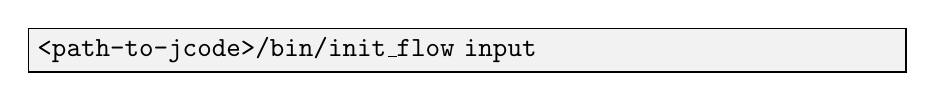
\begin{tikzpicture}
\node[draw, fill = gray!10,text width=0.9\textwidth] at (0,0) {\code{<path-to-jcode>/bin/init\_flow input}};
\end{tikzpicture}
\vspace{1em}
%\\\\
%\code{<path-to-jcode>/bin/init\_flow input}
%\\\\

%\\\\
%\vspace{1em}
%\begin{tikzpicture}
%\node[draw, fill = gray!10,text width=0.9\textwidth] at (0,0)
%{\begin{minipage}{\textwidth}
%\begin{verbatim}
%Simulation is 3D
%--------------------------------
%Grid size :  128 x   65 x    8 points
%min. Jacobian =  1.25E+04 at (   1,   33,    1)
%max. Jacobian =  2.97E+04 at (   1,    1,    1)
%\end{verbatim}
%\end{minipage}};
%\end{tikzpicture}

\noindent Relevant initialization information will be output to the screen. By default, this will create two new files:
\code{grid}, \code{data.init},
unless other names are specified in the \inp file. \jcode requires these two files to run the simulation. If particles or the immersed boundary method is enabled, additional files will be written during initialization.

\subsubsection*{Running}
To run the code on a single processor:
\\\\
\vspace{1em}
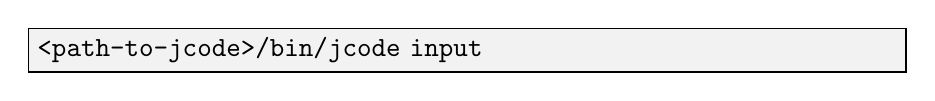
\begin{tikzpicture}
\node[draw, fill = gray!10,text width=0.9\textwidth] at (0,0) {\code{<path-to-jcode>/bin/jcode input}};
\end{tikzpicture}
\vspace{1em}
\\
To run with \code{<n>} processors:
\\\\
\vspace{1em}
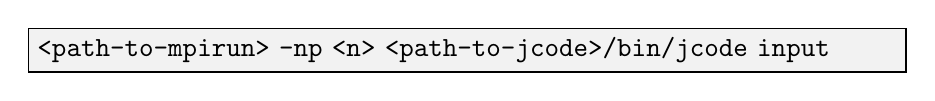
\begin{tikzpicture}
\node[draw, fill = gray!10,text width=0.9\textwidth] at (0,0) {\code{<path-to-mpirun> -np <n> <path-to-jcode>/bin/jcode input}};
\end{tikzpicture}
\vspace{1em}
\\
An example run with four processors will output the following to the screen:
\\\\
\vspace{1em}
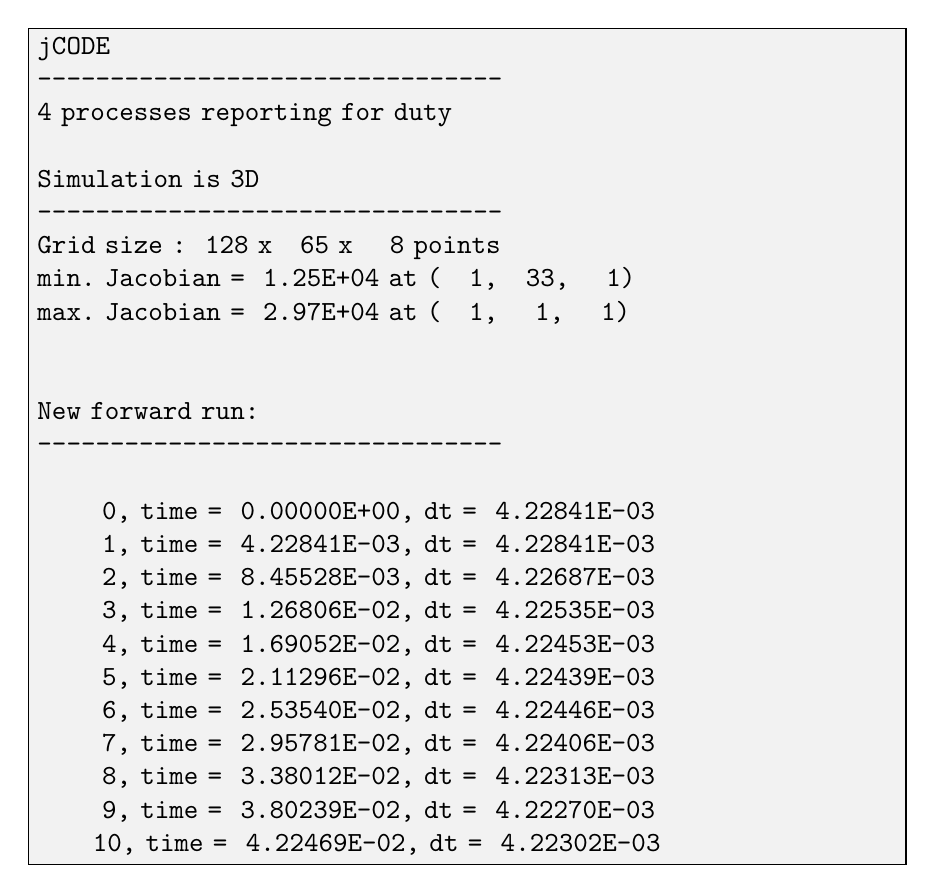
\begin{tikzpicture}
\node[draw, fill = gray!10,text width=0.9\textwidth] at (0,0)
{\begin{minipage}{\textwidth}
\begin{verbatim}
jCODE
--------------------------------
4 processes reporting for duty

Simulation is 3D
--------------------------------
Grid size :  128 x   65 x    8 points
min. Jacobian =  1.25E+04 at (   1,   33,    1)
max. Jacobian =  2.97E+04 at (   1,    1,    1)


New forward run:
--------------------------------

       0, time =  0.00000E+00, dt =  4.22841E-03
       1, time =  4.22841E-03, dt =  4.22841E-03
       2, time =  8.45528E-03, dt =  4.22687E-03
       3, time =  1.26806E-02, dt =  4.22535E-03
       4, time =  1.69052E-02, dt =  4.22453E-03
       5, time =  2.11296E-02, dt =  4.22439E-03
       6, time =  2.53540E-02, dt =  4.22446E-03
       7, time =  2.95781E-02, dt =  4.22406E-03
       8, time =  3.38012E-02, dt =  4.22313E-03
       9, time =  3.80239E-02, dt =  4.22270E-03
      10, time =  4.22469E-02, dt =  4.22302E-03
\end{verbatim}
\end{minipage}};
\end{tikzpicture}

\noindent The number of processors and grid diagnostics are first reported. This includes the number of grid points and the min/max Jacobian (corresponding to the min/max volume element). Next, the columns correspond to
\begin{itemize}
\item \# : number of the timestep
\item Time : running time of the simulation
\item dt/cfl : The minimum timestep or the maximum CFL, depending on the time stepping configuration
\end{itemize}
In addition, two directories have been created
\begin{itemize}
\item \code{monitor}: contains files to monitor the behavior of the code
\item \code{ensight-3D}: contains files used to visualize the flow field
\end{itemize}

%%%%%%%%%%%%%%%%%%%%%%%%%%%%%%%%%%%%%%%%%%%%%%%%%%%%%%
%%%%%%%%%%%%%%%%%%%%%%%%%%%%%%%%%%%%%%%%%%%%%%%%%%%%%%
%%%%%%%%%%%%%%%%%%%%%%%%%%%%%%%%%%%%%%%%%%%%%%%%%%%%%%
\subsection{Sod shock tube}
This case solves the one-dimensional Sod shock tube problem on a two-dimensional grid of size $401\times 32$. Characteristic boundary conditions are imposed in direction 1 and periodic boundary conditions imposed in direction 2. In addition, an absorbing sponge zone is included on the left and right boundaries. The pre- and post-shock density and pressure are specified under the \code{\# Initialization parameters}. Execute the following commands in the terminal to change to the appropriate directory, initialize, and run:
\\\\
\vspace{1em}
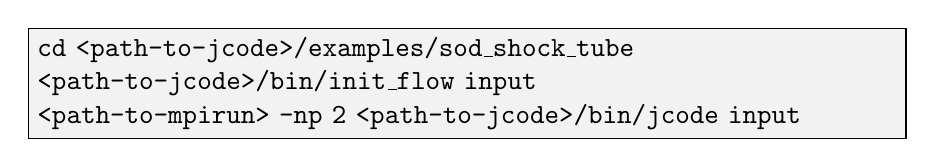
\begin{tikzpicture}
\node[draw, fill = gray!10,text width=0.9\textwidth] at (0,0) {
\code{cd <path-to-jcode>/examples/sod\_shock\_tube}\\
\code{<path-to-jcode>/bin/init\_flow input}\\
\code{<path-to-mpirun> -np 2 <path-to-jcode>/bin/jcode input}
};
\end{tikzpicture}
\vspace{.5em}
\\
The density profile at $t=0.2$ (400 time steps) should look like:
 \begin{figure}[h]
	\begin{center}
		\includegraphics[scale=0.5]{fig/sod_shock}
		\caption{Solution to the Sod shock tube example at $t=0.2$.}
		\label{fig:sod}
	\end{center}
\end{figure}

%Running the simulation with one processor will yield:
%\\\\
%\vspace{1em}
%\begin{tikzpicture}
%\node[draw, fill = gray!10,text width=0.9\textwidth] at (0,0)
%{
%\begin{minipage}{\textwidth}
%\begin{verbatim}
%jCODE
%--------------------------------
%   1 process reporting for duty
%
%Simulation is 2D
%--------------------------------
%  Grid size :  201 x   32 x    1 points
%    min. Jacobian =  4.00E+04 at ( 195,   17,    1)
%    max. Jacobian =  4.00E+04 at ( 199,   29,    1)
%
%
%New forward run:
%--------------------------------
%
%       0, time =  0.00000E+00, CFL =  1.67332E-01
%       1, time =  5.00000E-04, CFL =  1.89212E-01
%       2, time =  1.00000E-03, CFL =  2.14781E-01
%       3, time =  1.50000E-03, CFL =  2.31620E-01
%       4, time =  2.00000E-03, CFL =  2.43122E-01
%       5, time =  2.50000E-03, CFL =  2.51259E-01
%       6, time =  3.00000E-03, CFL =  2.57102E-01
%       7, time =  3.50000E-03, CFL =  2.61209E-01
%       8, time =  4.00000E-03, CFL =  2.63874E-01
%       9, time =  4.50000E-03, CFL =  2.65257E-01
%      10, time =  5.00000E-03, CFL =  2.65462E-01
%\end{verbatim}
%\end{minipage}};
%\end{tikzpicture}

\subsection{Particle-laden shock tube}
This case considers a shock interacting with a curtain of particles. The domain is of size $513\times 64$ with grid spacing $\Delta x = 2d_p$. The reference quantities correspond to air ($\rho_\infty^*=1.2$ kg/m$^3$, $\mu_\infty^*=1.8\times 10^{-5}$ Pa$\cdot$s, and $c_\infty^*=343$ m/s). The reference length corresponds to the particle diameter ($d_p=1$) with $L^*=100$ $\upmu$m. With this, the code Reynolds number is set to ${\rm Re}_c=2286.7$. Particles are initially randomly distributed within a thin layer in the pre-shock region of the domain. Particle collisions are turned on in this example, and the \code{collision time} is set to 10 (approximately $30\Delta t$). This example can be run by executing the following commands:
\\\\
\vspace{1em}
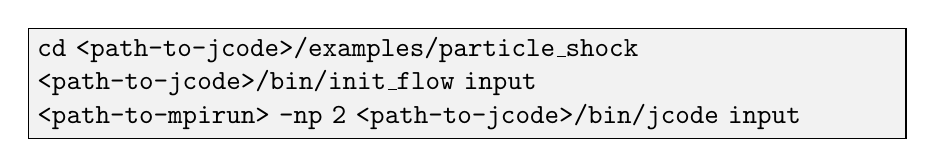
\begin{tikzpicture}
\node[draw, fill = gray!10,text width=0.9\textwidth] at (0,0) {
\code{cd <path-to-jcode>/examples/particle\_shock}\\
\code{<path-to-jcode>/bin/init\_flow input}\\
\code{<path-to-mpirun> -np 2 <path-to-jcode>/bin/jcode input}
};
\end{tikzpicture}
\vspace{.5em}
\\
After running \code{init\_flow} the code will write a particle file consisting of 684 particles randomly distributed within a thin layer in the middle of the domain with a mean volume fraction of 0.21. An instantaneous snapshot of particle position and Mach number at $t=660$ (after 1360 time steps):
 \begin{figure}[h]
	\begin{center}
		\includegraphics[scale=0.5]{fig/particle_shock}
		\caption{Particle shock interaction at $t=660$. Particle position (black), Mach number (color).}
		\label{fig:sod}
	\end{center}
\end{figure}

\subsection{Shock-wedge interaction using immersed boundaries}
The code has capabilities to account for complex geometries using a direct forcing immersed boundary method (IBM) adapted for compressible flows. The IBM enforces appropriate boundary conditions by placing discrete markers (particles) along the surface of the geometry and projecting a source term to neighboring grid points. Placement of the markers can be handled in two ways: (i) by analytically assigning the position to each marker; or (ii) automatic generation of the markers from a stereolythography (STL) file. A utility to convert STL files to the appropriate IBM file needed by the code is located in \code{/bin/stl2ibm}. The file \code{/src/utils/init\_flow/ibm\_init.f90} generates several canonical geometries analytically, including cylinders, plates, and wedges.

This case solves a shock passing a triangular wedge on a two-dimensional grid of size $513\times 415$. Characteristic boundary conditions are imposed at the left and right side of the domain, and slip-wall conditions are imposed at the top and bottom. In addition, an absorbing sponge zone is included on the left and right boundaries. 400 marker particles are placed along the sides of the wedge. It is important that there exists at least 1 marker per grid point (i.e., the average distance between marker particles should be less than $\Delta x$). The wedge position and size can be adjusted in the \code{input} file. This example can be run by executing the following commands:
\\\\
\vspace{1em}
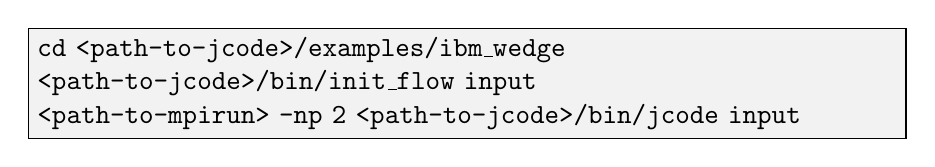
\begin{tikzpicture}
\node[draw, fill = gray!10,text width=0.9\textwidth] at (0,0) {
\code{cd <path-to-jcode>/examples/ibm\_wedge}\\
\code{<path-to-jcode>/bin/init\_flow input}\\
\code{<path-to-mpirun> -np 2 <path-to-jcode>/bin/jcode input}
};
\end{tikzpicture}
\vspace{.5em}
\\
During run time, additional files are generated to monitor the progress of the IBM (\code{monitor/ibm} and \code{monitor/ibm\_force}). If EnSight output is enabled, the IBM markers will automatically be dumped for visualization (as shown in blue in Fig.~\ref{fig:wedge}). Numerical schlieren at $t=5$ (750 time steps) should look like:
 \begin{figure}[h]
	\begin{center}
		\includegraphics[scale=0.35]{fig/ibm_wedge}
		\caption{Numerical schlieren of a shock-wedge interaction at $t=5$. IBM marker particles shown in blue.}
		\label{fig:wedge}
	\end{center}
\end{figure}

%\subsection{Premixed hydrogen flame}
%This case solves the one-dimensional Sod shock tube problem on a two-dimensional grid of size $401\times 32$. Characteristic boundary conditions are imposed in direction 1 and periodic boundary conditions imposed in direction 2. In addition, an absorbing sponge zone is included on the left and right boundaries. The pre- and post-shock density and pressure are specified under the \code{\# Initialization parameters}. Execute the following commands in the terminal to change to the appropriate directory, initialize, and run:
%\\\\
%\vspace{1em}
%\begin{tikzpicture}
%\node[draw, fill = gray!10,text width=0.9\textwidth] at (0,0) {
%\code{cd <path-to-jcode>/examples/sod\_shock\_tube}\\
%\code{<path-to-jcode>/bin/init\_flow input}\\
%\code{<path-to-mpirun> -np 2 <path-to-jcode>/bin/jcode input}
%};
%\end{tikzpicture}
%\vspace{.5em}
%\\
%The density profile at $t=0.2$ (400 time steps) should look like:
% \begin{figure}[h]
%	\begin{center}
%		\includegraphics[scale=0.5]{fig/sod_shock}
%		\caption{Solution to the Sod shock tube example at $t=0.2$.}
%		\label{fig:sod}
%	\end{center}
%\end{figure}

\subsection{Von Karman vortex street on a curvilinear grid}
This case solves a flow past a cylinder on a two-dimensional grid in polar coordinates. The grid is discretized with 257 grid points in the radial direction and 129 grid points in the azimuthal direction. `O-periodic' boundary conditions are enforced in the azimuthal direction by specifying \code{periodicity type in y : overlap} in the \code{input} file. In this example it is important to specify \code{curvilinear domain : .true.} in the \code{input} file. Execute the following commands in the terminal to change to the appropriate directory, initialize, and run:
\\\\
\vspace{1em}
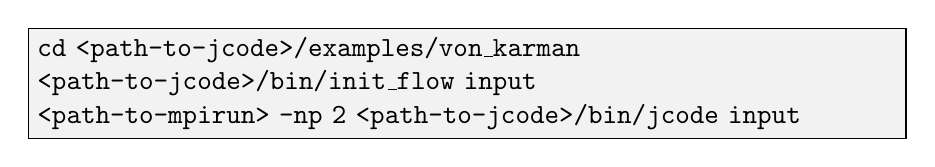
\begin{tikzpicture}
\node[draw, fill = gray!10,text width=0.9\textwidth] at (0,0) {
\code{cd <path-to-jcode>/examples/von\_karman}\\
\code{<path-to-jcode>/bin/init\_flow input}\\
\code{<path-to-mpirun> -np 2 <path-to-jcode>/bin/jcode input}
};
\end{tikzpicture}
\vspace{.5em}
\\
The Mach number at $t=68$ (3980 time steps) should look like:
 \begin{figure}[h]
	\begin{center}
		\includegraphics[scale=0.3]{fig/von_karman}
		\caption{Von K\`arm\`an vortex street using curvilinear coordinates.}
		\label{fig:sod}
	\end{center}
\end{figure}

%%%%%%%%%%%%%%%%%%%%%%%%%%%%%%%%%%%%%%%%%%%%%%%%
%%%%%%%%%%%%%%%%%%%%%%%%%%%%%%%%%%%%%%%%%%%%%%%%
%%%%%%%%%%%%%%%%%%%%%%%%%%%%%%%%%%%%%%%%%%%%%%%%
\subsection{Adjoint sensitivity of an acoustic monopole}
This case solves a two-dimensional flow with acoustic forcing and the corresponding adjoint sensitivity. The gradient accuracy of the adjoint sensitivity is compared with a finite difference approximation. The cost functional is defined as the time-integrated pressure fluctuations within a specified target region. A source term on the right-hand-side of the energy equation is adjusted to act as a controller. The \code{cost functional type} is \code{sound} and \code{controller type} is \code{thermal actuator}. Parameters to adjust the location and extent of the target region and control region can be found under \code{\# Adjoint parameters} in the \code{input} file. Execute the following commands in the terminal to change to the appropriate directory, initialize, and run:
\\\\
\vspace{1em}
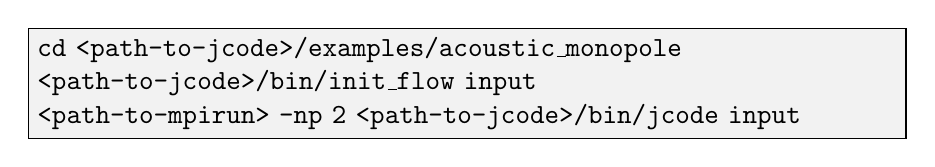
\begin{tikzpicture}
\node[draw, fill = gray!10,text width=0.9\textwidth] at (0,0) {
\code{cd <path-to-jcode>/examples/acoustic\_monopole}\\
\code{<path-to-jcode>/bin/init\_flow input}\\
\code{<path-to-mpirun> -np 2 <path-to-jcode>/bin/jcode input}
};
\end{tikzpicture}
\vspace{.5em}
\\
The code will initially perform a `forward run', i.e. a baseline prediction with zero actuation. During this run the instantaneous and time-integrated cost functional are output to \code{monitor/functional}. Once the baseline run is complete, the adjoint equations are solved backward in time. During this time, sensitivity information is written to \code{monitor/adjoint\_sensitivity} and \code{monitor/adjoint\_timing}. In this example, the control forcing is a function of space and time, and its values are saved to \code{gradient\_controlRegion.dat} as a binary file. Once the adjoint solution is complete, a steepest-descent is performed by running several forward runs with varying actuation amounts. This is done to perform a finite difference estimation of the sensitivity gradient. New files are written to the \code{monitor} directory during each iteration. The gradient accuracy information is written to \code{gradient\_error.txt}. This file contains the actuation amount (i.e. the finite difference step size), cost functional, cost sensitivity, and the gradient error for each iteration. The error is shown in Fig.~\ref{fig:gradient_accuracy}.
\begin{figure}[h!]
\centering
\begin{subfigure}[b]{0.44\textwidth}
\includegraphics[width=\linewidth]{fig/acoustic_pressure.png}
\caption{}
%\label{fig:}
\end{subfigure}
\begin{subfigure}[b]{0.44\textwidth}
\includegraphics[width=\linewidth]{fig/gradient_error.png}
\caption{}
\label{fig:gradient_accuracy}
\end{subfigure}
\caption{(\textit{a}) Pressure distribution for acoustic monopole at simulation time 24, (\textit{b}) gradient accuracy of the adjoint sensitivity}
\label{fig:my_label}
\end{figure}

%%%%%%%%%%%%%%%%%%%%%%%%%%%%%%%%%%%%%%%%%%%%%%%%
%%%%%%%%%%%%%%%%%%%%%%%%%%%%%%%%%%%%%%%%%%%%%%%%
%%%%%%%%%%%%%%%%%%%%%%%%%%%%%%%%%%%%%%%%%%%%%%%%
\newpage
\appendix
\begin{appendices}

\section{Drag laws used in \code{jCODE}}\label{app:drag}
\subsection{Basic form -- the drag coefficient and the superficial velocity}
Let's consider fluid with viscosity $\mu$ and density $\rho$ flowing with velocity $\bm{u}$ past a solid spherical particle with velocity $\bm{u}_p$, diameter $d_p$, and density $\rho_p$. The drag coefficient is defined as
\begin{equation}\label{eq:Cd}
C_D=\frac{\bm{f}_{\rm drag}}{\frac{1}{2}\rho\|\bm{v}_r\|\bm{v}_r A},
\end{equation}
where $\bm{f}_{\rm drag}$ is the drag force appearing in \eqref{eq:finter}, $\bm{v}_r=\alpha(\bm{u}-\bm{u}_p)$ is the \textit{superficial} relative velocity, with $\alpha$ the fluid volume fraction, and $A=\pi d_p^2/4$ is the frontal area of the particle. The superficial velocity attempts to approximate the local velocity as if the particle was not there. In general, the fluid velocity can be expressed as $u=Q/A$, where $Q$ is the volume flow rate of the fluid, and $A$ is the cross sectional area under consideration. For an incompressible flow, $Q$ will change according to the area change. Thus, for a flow moving with velocity $u$ through a suspension of particles with volume fraction $\alpha$, the superficial velocity can be determined by equating $Q=u_1A_1=u_2A_2$, where $u_1=u$ is the actual velocity, $A_1=\alpha A$ is the area the fluid is flowing through, $u_2=u_s$ is the velocity we desire through $A_2=A$, the area in the absence of particles. Thus, the superficial velocity is $u_s=\alpha u$.

The following section will define different drag models available in \code{jCODE}, which are used to update the particle position (assuming spherical particles) according to
\begin{equation}\label{eq:dudt}
%\frac{{\rm d}\bm{u}_p}{{\rm d}t}=\frac{3}{4}\frac{\rho}{\rho_p}\frac{C_D\|\bm{v}_r\|\bm{v}_r}{d_p}=K\bm{v}_r\quad\text{with}\quad K=\frac{3}{4}\frac{\rho}{\rho_p}\frac{C_D\|\bm{v}_r\|}{d_p}.
\frac{{\rm d}\bm{u}_p}{{\rm d}t}=\frac{F_D}{\tau_p}\alpha\left(\bm{u}-\bm{u}_p\right)\quad\text{with}\quad F_D=\frac{\Rep}{24}C_D,
\end{equation}
where $\tau_p=\rho_p d_p^2/(18\mu)$ is the particle response time (valid in the Stokes regime), $\Rep=\rho d_p\|\bm{v}_r\|/\mu$ is the particle Reynolds numbers, and $F_D=F_d(\Rep,\alpha,\text{etc.})$ is a non-dimensional correction to Stokes drag.

\subsection{\code{Stokes}~\cite{stokes1851effect}}
In 1851, Sir George Gabriel Stokes derived the drag force for an isolated particle in a low Reynolds number flow, which is given by
\begin{equation}
\bm{F}_d^{\rm Stokes}=3\pi d_p\mu\bm{v}_r.
\end{equation}
This expression can be rearranged to form an acceleration: $\bm{F}_D/m_p=\bm{v}_r/\tau_p$, where $m_p=\rho_p d_p^3/6$ is the particle mass. Using \eqref{eq:Cd} and \eqref{eq:dudt}, this expression can be rearranged to form the drag coefficient in the Stokes limit:
\begin{equation}
C_D = \frac{24}{\Rep}\quad \text{and thus}\quad F_D=1.
\end{equation}

\subsection{\code{Schiller-Naumann}~\cite{schiller1933fundamental}}
When ${\rm Re}_p>1$ and the flow is sufficiently dilute (i.e., $\alpha\approx 1$), Schiller and Naumann (1933)~\cite{schiller1933fundamental} derived an expression for the drag coefficient expressed as
\begin{equation}
C_D=\frac{24}{\Rep}\left(1+0.15\Rep^{0.687}\right) \quad {\rm and}\quad F_D=1+0.15\Rep^{0.687}.
\end{equation}

\subsection{\code{Gidaspow}~\cite{gidaspow1994multiphase}}
Dimitri Gidaspow's 1994 textbook~\cite{gidaspow1994multiphase} presents an expression for the drag force that varies with both the local Reynolds number and volume fraction for applications to fluidized beds. When $\alpha\le0.8$ (i.e., for dense suspensions), the formulation presented by Ergun~\cite{ergun1952fluid} is employed, whereas the formulation by Wen \& Yu~\cite{wen1966mechanics} is used when $\alpha>0.8$ (i.e., for dilute suspensions):
\begin{equation}
\beta=\begin{cases}
    150\frac{\alpha_p^2\mu}{\alpha d_p^2}+1.75\frac{\rho\alpha_p\bm{v}_r}{\alpha d_p}, & \alpha\le 0.8\\
    \frac{3}{4} C_D \frac{\rho\alpha_p\bm{v}_r}{d_p}\alpha^{-2.65}, & \alpha > 0.8,
  \end{cases} \quad
\end{equation}
with
\begin{equation}
C_D=\begin{cases}
    \frac{24}{\Rep}\left(1+0.15\Rep^{0.687}\right), & \Rep<1000\\
    0.44, & \Rep\ge1000.
  \end{cases} \quad
\end{equation}
The interphase coefficient $\beta$ is related to $F_D$ according to
\begin{equation}
F_D=\frac{\tau_p\beta}{\rho_p\alpha_p}.
\end{equation}

\subsection{\code{Tenneti}~\cite{tenneti2011drag}}
In more recent years, particle-resolved direct numerical simulations (PR-DNS) have been used to develop improved drag laws. The drag law of Tenneti et al.~\cite{tenneti2011drag} is valid for $0\le\alpha\le0.5$ and $0\le\Rep\le300$. It reduces to \code{Schiller-Naumann} in the limit $\alpha\rightarrow0$ and \code{Stokes} when $\Rep\rightarrow0$. The non-dimensional drag correction is given by
\begin{equation}
F_D=\frac{1+0.15\Rep^{0.687}}{\alpha^2}+b_1(\alpha)+b_2(\alpha,\Rep),
\end{equation}
where
\begin{equation}
b_1=\frac{5.81\alpha_p}{\alpha^2}+\frac{0.48\alpha_p^{1/3}}{\alpha^3}\quad\text{and}\quad b_2=\alpha\alpha_p^3\Rep\left(0.95+\frac{0.61\alpha_p^3}{\alpha^2}\right).
\end{equation}
It should be noted that there is an extra factor of $\alpha$ appears in this expression compared to the original paper to remove the contribution of the mean pressure gradient used in the PR-DNS.
\end{appendices}

%%%%%%%%%%%%%%%%%%%%%%%%%%%%%%%%%%%%%%%%%%%%%%%%
%%%%%%%%%%%%%%%%%%%%%%%%%%%%%%%%%%%%%%%%%%%%%%%%
%%%%%%%%%%%%%%%%%%%%%%%%%%%%%%%%%%%%%%%%%%%%%%%%
\newpage
\bibliography{references}
\bibliographystyle{unsrt}

\end{document}